%======================================================================================================
%======================================================================================================
% PLANTILLA PARA INFORMES T�CNICOS de la DAS de la DIIV
%  Versi�n 1.4 del 21/1/2019
%	-Utilizaci�n de hoja de estilo para facilitar incorporar paquetes y comandos.
% 	-Rearmado de portada. Mayor sobriedad y destaque del t�tulo del informe t�cnico.
%	-Incorporados fixes varios para poder referir secciones y que no aparezcan '.' al final.
%	-Incorporado par�metro para que no se estire hasta el final los �tems del glosario.
%	-Afectada la geometr�a: tiene menor margen en toda direcci�n.
%	-Cambio de color rojo a negro t�tulos varios.
%	-Modificado apa-good.bst --> italizado el "et al"
%======================================================================================================
%======================================================================================================


% =====================================================================================================
% =====================================================================================================
% PRE�MBULO
% =====================================================================================================
% =====================================================================================================

\documentclass[11pt]{article}
\usepackage[T1]{fontenc} % para que pueda partir palabras con acentos
\usepackage[latin1]{inputenc}
\usepackage{rotating}
\usepackage{graphicx}
\usepackage[spanish]{babel} % Ojo que esto cambia el nombre de las secciones
\usepackage{times,url}
\usepackage{amsmath}
\usepackage{mathrsfs}
\usepackage{amsfonts}
\usepackage{amssymb}
%\usepackage{hyphen}
%\hyphenation{T-6 T-7 LEAD\_RESISTANCE}
\usepackage{fullpage}
\usepackage{pdflscape}

\usepackage[a4paper,bottom=2.7cm,top=2.7cm,left=2.5cm,right=2.5cm]{geometry}
\usepackage{fancyhdr} % Esto cambiar� la ubicaci�n de los numeritos de las p�ginas
\usepackage{grffile} % Para tipear nombres de archivo con espacios
%\usepackage{esvect} % Para poner flechas de vector m�s copadas
\usepackage{array} % Paquete que mejora la funcionalidad de array

% Carga de paquetes extra
\usepackage{color}
\usepackage{colortbl}
\usepackage{tocloft}
\usepackage{setspace}
\usepackage{titlesec}
\usepackage{fix-cm}
\usepackage{natbib}
\setcitestyle{square}
\usepackage{multirow}
\usepackage{bigstrut}

\usepackage{wrapfig}
\usepackage{enumitem}
\usepackage{appendix}

% Se carga la hoja de estilo
\usepackage{RT_estilo} 
\usepackage{fancyvrb}

% Fracciones bonitas
\usepackage{nicefrac}

% =====================================================================================================
% =====================================================================================================
%
% DOCUMENTO PROPIAMENTE DICHO
%
% =====================================================================================================
% =====================================================================================================

\begin{document}

% =====================================================================================================
% =====================================================================================================
% PORTADA
% =====================================================================================================
% =====================================================================================================
\thispagestyle{empty}

%	==============================================================
%	Caja Superior
%	==============================================================

	\noindent
	\begin{minipage}[c][50mm][c]{1.0\linewidth} 
		\begin{center}
			\Large{\textbf{\underline{PROYECTO}:}}\\
			\vspace{2mm}
			\Large{\textbf{ MODERNIZACI�N Y DIGITALIZACI�N DEL SISTEMA DE REGISTRO DE TRAZOS BATITERMOGR�FICOS XBT DE LAS UNIDADES DE SUPERFICIE DEL COMANDO DE LA FLOTA DE MAR.}}\\
			\vspace{2mm}		
			\textbf{Direcci�n del proyecto:}\hspace{2pc}\textit{Patricio Bos}\\
			\textbf{Co-Direcci�n del proyecto:}\hspace{2pc}\textit{Christian Galasso}\\
		\end{center}
	\end{minipage}
	\vspace{1mm}

%	============================================================== 
% 	Caja Central
%	==============================================================

	\noindent
	\begin{minipage}[c][70mm][c]{1.0\linewidth} 
		\textcolor{coolblack}{\hrule\hrule}
% 		\vspace{1mm}
% 		\textcolor{blue}{\hrule\hrule}
 		\vspace{5mm}
		\begin{flushleft}
			\huge{Dise�o e implementaci�n de etapa de acondicionamiento de se�al para sistema XBT}\\
	 		\vspace{5mm}
%			\Large{EN ELABORACI�N}
		\end{flushleft}
		\vspace{8mm}
		\begin{flushright}
			\Large{Patricio Bos, Mariano Cinquini}\\
		\end{flushright}
		\vspace{2mm}
		\textcolor{coolblack}{\hrule\hrule}
% 		\vspace{1mm}
% 		\textcolor{blue}{\hrule\hrule}
	\end{minipage}
	\vspace{-5mm}

	\noindent
	\begin{minipage}[c][30mm][c]{1.0\linewidth} 		
		\begin{flushright}
			\Large{Divisi�n Ac�stica Submarina\\
				Informe T�cnico AS 07/22\\
				Julio 2022}\\
		\end{flushright}
	\end{minipage}
	\vspace{5mm}
	
%	==============================================================	
% 	Caja inferior
%	==============================================================

	\noindent
	\begin{minipage}[c][60mm][c]{1.0\linewidth} 
% 		\begin{table}[h]
			\begin{minipage}[c]{0.35\linewidth}
				\centering
				
\includegraphics[width=3cm]{graficos/ESCUDO.jpg}
			\end{minipage}
			\hspace*{1pc}\hfill
			\begin{minipage}[c]{0.60\linewidth}
				\begin{center}
					\Huge{\textbf{DIIV}}\\
					\Large{DIRECCI�N DE\\ 
					INVESTIGACI�N DE LA ARMADA}\\
				\end{center}
			\end{minipage}			
			\begin{minipage}[c]{1.0\linewidth}
				\hfill\vspace{4mm}
			\end{minipage}
			\begin{minipage}[c]{0.35\linewidth}
				\centering
				
\includegraphics[width=5cm]{graficos/LOGO_UNIDEF_SOLO.jpg}
			\end{minipage}
			\hspace*{1pc}\hfill
			\begin{minipage}[c]{0.60\linewidth}
				\begin{center}
					\Huge{\textbf{UNIDEF}}\\					
					\Large{UNIDAD EJECUTORA DE\\
					INVESTIGACI�N Y DESARROLLO\\
					ESTRAT�GICOS PARA LA DEFENSA}\\
					CONICET/MINDEF\\
				\end{center}
			\end{minipage}
% 		\end{table}
	\end{minipage}		

\clearpage


% \thispagestyle{empty}
% % \vspace*{\fill}
% %%%%%%%%%%%%%%%%%%%%%%%%%%%%%%%%%%%%%%%%%%%%%%%%%%%%%%%%
% % Estructura para el t�tulo de proyecto y los directores
% %%%%%%%%%%%%%%%%%%%%%%%%%%%%%%%%%%%%%%%%%%%%%%%%%%%%%%%%
% 		\begin{table*}[h]
% 			\centering
% 			%\vfill
% 			\begin{center}
% 					\Large{\textbf{\textcolor{black}{\underline{PROYECTO}:}}}\\
% 					\vspace{0.20pc}
% 					\Large{\textbf{\textcolor{black}{para PERMITIR ANIDAR Y FRACTURAR.}}}\\
% 					\vspace{1pc}		
% 					\textbf{Direcci�n del proyecto:}\hspace{3pc}\textit{Director}\\
% 					\textbf{Co-Direcci�n del proyecto:}\hspace{3pc}\textit{Codirector}\\									
% 			\end{center}
% 		\end{table*}
% 		\vspace{20mm}
% %%%%%%%%%%%%%%%%%%%%%%%%%%%%%%%%%%%%%%%%%%%%%%%%%%%%%%%%
% % Estructura para el t�tulo del trabajo
% %%%%%%%%%%%%%%%%%%%%%%%%%%%%%%%%%%%%%%%%%%%%%%%%%%%%%%%%				
% 		\begin{table*}[h]
% 				\centering
% 				%\vfill
% 				\begin{center}
% 						\fcolorbox{blue}{white}{
% 							\fcolorbox{blue}{white}{
% 		         				\begin{minipage}[t]{0.65\textwidth}
%         							\begin{center}
% 										\textbf{\textcolor{blue}{\Large{T�tulo del trabajo que podr�a llegar a tener otro rengl�n.}}}\\
% 										\vspace{0.5pc} 
% 									  	\textbf{\textcolor{blue}{por}}\\
% 									  	\vspace{0.5pc}	
% 										\textbf{\it \textcolor{blue}{Autor 1, Autor 2 y Autor 
% 3}}\\		
% 									\end{center}
%          						\end{minipage}
%       							}
%    						}
% 				\end{center}
% 		\end{table*}	
% %%%%%%%%%%%%%%%%%%%%%%%%%%%%%%%%%%%%%%%%%%%%%%%%%%%%%%%%
% % Estructura para el logo y la pertenencia a instituciones
% %%%%%%%%%%%%%%%%%%%%%%%%%%%%%%%%%%%%%%%%%%%%%%%%%%%%%%%%		
% 		\vspace{-9mm}
% 		\begin{flushright}
% 				\large{Divisi�n Ac�stica Submarina\\
% 					Informe T�cnico AS 1/12\\
% 					Febrero 2012}\\
% 		\end{flushright}
% 		\vspace{30mm}
% 		\begin{table*}[h]
% 			\begin{minipage}[c]{0.39\linewidth}
% 				\centering
% 				\frame{
\includegraphics[width=0.55\textwidth]{graficos/ESCUDO.jpg}}
% 			\end{minipage}
% 			\hspace*{1pc}
% 			\begin{minipage}[c]{0.60\linewidth}
% 				\begin{center}
% 					\Huge{\textbf{DIIV}}\\
% 					\Large{DIRECCI�N DE\\ 
% 					INVESTIGACI�N DE LA ARMADA}\\
% 				\end{center}
% 			\end{minipage}			
% 			\begin{minipage}[c]{1.0\linewidth}
% 				\hfill\vspace{4mm}
% 			\end{minipage}
% 			\begin{minipage}[c]{0.40\linewidth}
% 				\centering
% 				\frame{
\includegraphics[width=1.0\textwidth]{graficos/LOGO_UNIDEF_SOLO.jpg}}
% 			\end{minipage}
% 			\hspace*{1pc}
% 			\begin{minipage}[c]{0.60\linewidth}
% 				\begin{center}
% 					\Huge{\textbf{UNIDEF}}\\					
% 					\Large{UNIDAD EJECUTORA DE\\
% 					INVESTIGACI�N Y DESARROLLO\\
% 					ESTRAT�GICOS PARA LA DEFENSA}\\
% 					CONICET/MINDEF\\
% 				\end{center}
% 			\end{minipage}
% 		\end{table*}
% % \vspace*{\fill}
% \clearpage


% =====================================================================================================
% =====================================================================================================
% P�GINA DE RESUMEN EN CASTELLANO Y EN INGL�S
% =====================================================================================================
% =====================================================================================================

\begin{center}
	\large{\textbf{\textcolor{black}{Dise�o e implementaci�n de etapa de acondicionamiento de se�al para sistema XBT}}}\\
	\vspace{1pc}
	\textbf{Autor 1, Autor 2 y Autor 3}
\end{center}

\bigskip
	\begin{center}
		\textcolor{black}{RESUMEN}	
	\end{center}
	\begin*
		\indent
		\textit{Escriba aqu� el resumen en castellano.}
	\end*

\bigskip
	\begin{center}
		\textcolor{black}{ABSTRACT}
	\end{center}
	\begin*
		\indent
		\textit{Type here your abstract in english.} 
	\end*

\clearpage

% =====================================================================================================
% =====================================================================================================
% P�GINA DESCRIPTIVA DE PERTENENCIA A PROYECTO DEL TRABAJO
% =====================================================================================================
% =====================================================================================================

\vspace*{170pt}

\begin{center}
	\begin{tabular}[c]{c}
% 		\arrayrulecolor{red}
		\hline\hline
		\\
		\Large{Este trabajo es parte del Proyecto}\vspace{2mm}\\
		\Large{MODERNIZACI�N Y DIGITALIZACI�N DEL SISTEMA DE}\vspace{1mm}\\
		\Large{REGISTRO DE TRAZOS BATITERMOGR�FICOS XBT DE LAS}\vspace{2mm}\\
		\Large{UNIDADES DE SUPERFICIE DEL COMANDO DE LA FLOTA DE MAR.}\vspace{2mm}\\
		\Large{del Programa UNDEFI de la Universidad de la Defensa Nacional,}\vspace{2mm}\\ 
		\Large{que se lleva a cabo en la Divisi�n Ac�stica Submarina}\vspace{2mm}\\ 
		\Large{de la Direcci�n de Investigaci�n de la Armada (DIIV) de la}\vspace{2mm}\\ 
		\Large{Direcci�n General  de Investigaci�n y Desarrollo de la Armada (DGID).}\vspace{2mm}\\
		\\
		\hline\hline
	\end{tabular}
\end{center}

\clearpage





% =====================================================================================================
% =====================================================================================================
% P�GINA DE AGRADECIMIENTOS
% =====================================================================================================
% =====================================================================================================
% La configuraci�n est� optimizada para fotos de 3cm de ancho (arm�nicamente).  
%


\begin{center}
	\Large\textbf{{\textcolor{black}{AGRADECIMIENTOS}}}
\end{center}Los autores desean expresar su agradecimiento a:

\vspace{2pc}


\begin{minipage}[c]{0.2\linewidth}
	\frame{
\includegraphics[width=0.7\textwidth]{graficos/Alonso.pdf}}
\end{minipage}
\hfill
\begin{minipage}[c]{0.75\linewidth}
Ing. Jos� Luis Alonso, jefe de secci�n del Taller de Electr�nica del Arsenal Naval Puerto Belgrano (TEAP) por su gentileza al facilitar informaci�n sobre los sistemas batitermogr�ficos Sippican y por permitir el acceso al taller a su cargo para realizar ensayos relacionados con el proyecto. Asimismo, se deja constancia de su permanente apoyo, colaboraci�n y entusiasmo por el tema abordado.
\end{minipage}%\vfill
\vspace{2pc}
\clearpage

% =====================================================================================================
% =====================================================================================================
% �NDICE
% =====================================================================================================
% =====================================================================================================


\tableofcontents
\clearpage


% =====================================================================================================
% =====================================================================================================
% GLOSARIO DE SIGLAS
% =====================================================================================================
% =====================================================================================================


\begin{center}
	\Large\textbf{{\textcolor{black}{GLOSARIO DE SIGLAS}}}
\end{center}
\begin{tabular}{l p{12cm}}
	ADC		&	Analog to Digital Converter (Conversor Anal�gico Digital) \\	
	APS		&	Alcance Predicho SONAR\\	
	ARA		&	Armada Argentina\\
	COAN	&	Comando de Aviaci�n Naval\\
	COFM	&	COmando de la Flota de Mar\\
	COFS	&	COmando de Fuerza de Submarinos\\
	DAC		&	Digital to Analog Converter (Conversor Digital Anal�gico) \\	
	DAS		&	Divisi�n Ac�stica Submarina de la DIIV\\
	DPA		&	Departamento de Propagaci�n Ac�stica\\
	DGID	&	Direcci�n General de Investigaci�n y Desarrollo de la Armada\\
	DIIV	&	Direcci�n de Investigaci�n de la Armada\\
	JFET	&	Juntion Field Effect Transistor\\
	MAD		&	Modo Activo Directo\\	
	MEF		&	M�quina de Estados Finitos\\
	NTC		&	Negative Temperature Coefficient\\
	PCB		&	Printed Circuit Board (Placa de Circuito Impreso)\\
%	PNP		&	Transistor bipolar de juntura tipo PNP\\	
	SONAR	&	SOund Navigation And Ranging\\
	TEAP	&	Taller de Electr�nica del Arsenal Naval Puerto Belgrano\\
	TBJ		&	Transitor Bipolar de Juntura\\
	TL		&	Transmission Loss\\
	UNDEF	&	Universidad de la Defensa Nacional\\
	UNDEFi	&	Programa de acreditaci�n y financiamiento de proyectos de Investigaci�n y Desarrollo de la Universidad de la Defensa Nacional\\
	XBT		&	eXpendable BathyThermograph\\
\end{tabular}

\clearpage

% =====================================================================================================
% =====================================================================================================
% LISTA DE FIGURAS
% =====================================================================================================
% =====================================================================================================

\begin{center}
\listoffigures
\end{center}
\clearpage

% =====================================================================================================
% =====================================================================================================
% LISTA DE TABLAS
% =====================================================================================================
% =====================================================================================================

\begin{center}
\listoftables
\end{center}
\clearpage

% =====================================================================================================
% =====================================================================================================
% CUERPO DEL INFORME
% =====================================================================================================
% =====================================================================================================

\section{INTRODUCCI�N}

Un batiterm�grafo descartable, XBT por sus siglas en ingl�s (eXpendable BathyThermograph), es un instrumento utilizado por la Armada Argentina para medir el perfil de temperatura de parte de la columna de agua en navegaci�n sin afectar las condiciones de operaci�n del buque. El sistema que se utiliza actualmente en el Comando de la Flota de Mar (COFM) fue desarrollado en la d�cada de los setentas por la firma Sippican Inc., hoy subsidiaria de Lockheed Martin. El sistema est� formado por tres componentes:

\begin{itemize}
\item sondas batitermogr�ficas descartables para medir temperatura;
\item un lanzador para el despliegue de las sondas; y
\item un graficador de aguja anal�gico que imprime los resultados en una tira de papel graduado.
\end{itemize}

En la figura \ref{sistemaXBT} se puede observar un diagrama esquem�tico con las tres unidades que componen el sistema, tomada del manual \citep{sippican}.

\begin{figure}[htpb]
\centering
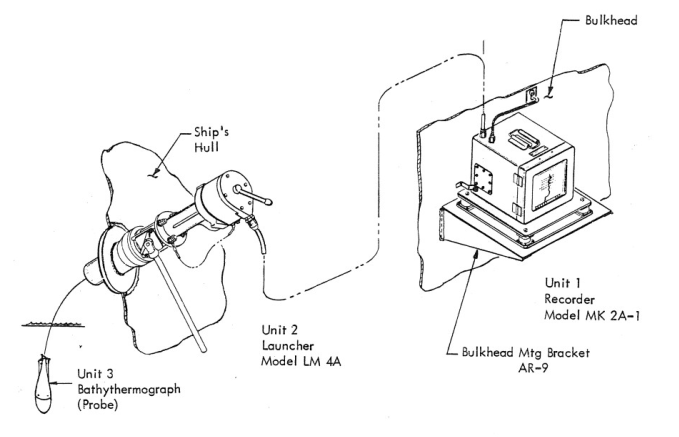
\includegraphics[width=.9\textwidth]{graficos/sistemaXBT.png}
\caption{Diagrama esquem�tico con los componentes del sistema XBT}
\label{sistemaXBT}
\end{figure}

Los XBTs se utilizan abordo de las unidades de superficie del COFM para determinar el perfil de la temperatura en funci�n de la profundidad y consecuentemente, para poder calcular la profundidad de napa o inicio de la termoclina, la velocidad �ptima SONAR y el perfil de velocidad del sonido, c(z), en la columna de agua, el Alcance Predicho SONAR (APS), las P�rdidas por Transmisi�n ac�stica (TL), entre otros par�metros de inter�s ac�stico.

En particular, la velocidad del sonido se calcula a partir de datos de temperatura y salinidad medidos \textit{in-situ}, o en su defecto, a partir de estimaciones estad�sticas existentes en bases de datos. Los perfiles de velocidad de sonido, c(z), constituyen un dato de entrada (\textit{input}) necesario en los sistemas automatizados (software propietario) de predicci�n de Alcance SONAR, provistos por el Dpto. Propagaci�n Ac�stica de la DIIV para usuarios de tres Comandos de la ARA, a saber: el Comando de la Flota de Mar (COFM), el Comando de Aviaci�n Naval (COAN) y el Comando de la Fuerza de Submarinos (COFS).

La predicci�n del APS es un t�pico de car�cter clasificado para todas las Armadas debido a su aplicaci�n directa a la detecci�n ac�stica en el mar para el �mbito de la guerra antisubmarina. El c�lculo del APS para una dada posici�n geogr�fica, en cierta fecha, se lleva a cabo sobre la base de varios elementos: 

\begin{enumerate}
	\item el perfil de velocidad de sonido, c(z), el cual a su vez exige el datos medido de temperatura en funci�n de la profundidad, T(z);
	\item informaci�n asociada al equipamiento electroac�stico del sistema fuente-receptor;
	\item condiciones meteorol�gicas;
	\item una compleja modelaci�n f�sica, que es responsabilidad de los investigadores del Departamento Propagaci�n Ac�stica de la DIIV pero que es un componente encapsulado y ``transparente'' para el usuario operativo naval.
\end{enumerate}

\section{DESCRIPCI�N FUNCIONAL DEL REGISTRADOR SIPPICAN MK 2A-1}

La l�gica de funcionamiento del sistema de registros batitermogr�ficos se encuentra contenido en la unidad de registro MK 2A-1.  Esta unidad cuenta con una fuente de alimentaci�n valvular, circuitos anal�gicos para acondicionar la se�al proveniente de la sonda XBT y componentes electromec�nicos para controlar una pluma o \textit{stylus} y el avance del papel graduado, a fin de imprimir el pefil de temperatura medido. 

El sistema XBT opera en cuatro modos de funcionamiento, RELOAD, CHECK/RUN, LAUNCH y MEASSURE.  Cuando se enciende el registrador se deben esperar 10 minutos para que el registrador entre en r�gimen.

En el modo RELOAD, el sistema espera que se inserte una (nueva) sonda batitermogr�ficas descartable en el lanzador.

Cuando se cierra la compuerta del lanzador con una sonda batitermogr�fica dentro, el sistema pasa al modo CHECK/RUN.  En este modo, el registrador funciona durante unos segundos posiciona la pluma del impresor en la temperatura de calibraci�n, 16,6 $^{\circ}$C. Inmediantamente despu�s, el sistema pasa al modo LAUNCH y queda a la espera del lanzamiento de la sonda.

Cuando la sonda batitermogr�ficas descartable es lanzada y toma contacto con el agua de mar, el sistema pasa al modo MEASSURE, donde se registra la temperatura de la columna de agua durante un tiempo fijo. Pasado ese tiempo, el registrador se detiene y el sistema pasa al modo RELOAD.

\subsection{Controles e indicadores}

El registrador MK 2A-1 cuenta con dos indicadores lum�nicos, RELOAD y LAUNCH y dos llaves, RECYCLE y 94$^{\circ}$ - 30$^{\circ}$, a los que se accede al abrir la tapa frontal, como se puede apreciar en la figura \ref{indicadoresXBT}.

\begin{figure}[htpb]
\centering
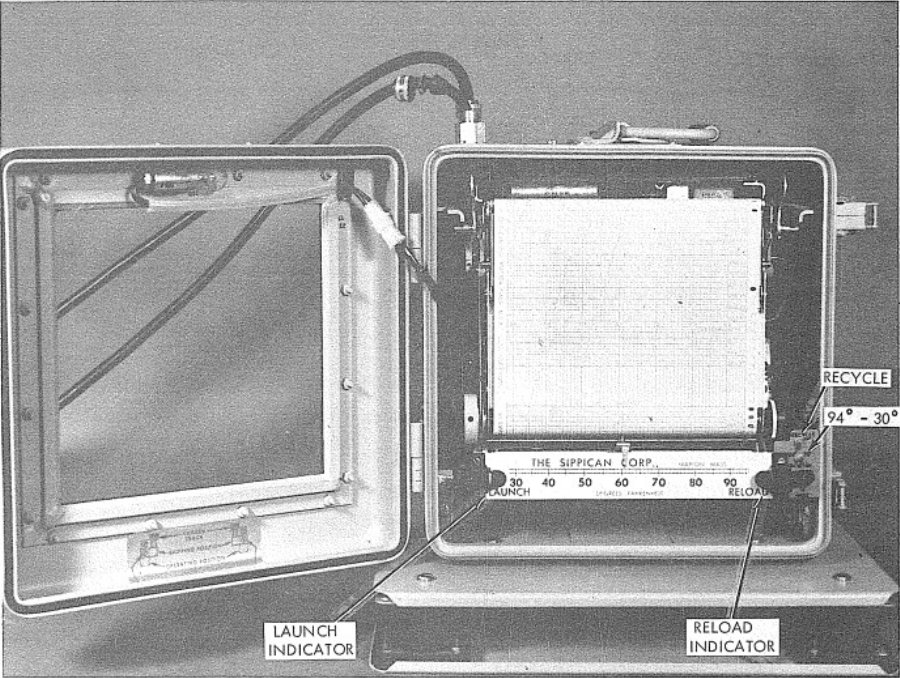
\includegraphics[width=.85\textwidth]{graficos/MK2A-1_indicadores.png}
\caption{Vista frontal del registrador MK 2A-1 con la ubicaci�n de los indicadores y controles.}
\label{indicadoresXBT}
\end{figure}

\begin{itemize}
\item RELOAD. Es un indicador lum�nico de color rojo, ubicado abajo a la derecha y es visible a trav�s del vidro de la puerta del registrador. Se enciende cuando el sistema est� preparado para que se inserte una sonda XBT en el lanzador.
\item LAUNCH. Es un indicador lum�nico de color verde, ubicado abajo a la izquierda y tambi�n es visible a trav�s del vidrio de la puerta del registrador. Se enciende cuando una sonda XBT ha sido insertada en el lanzador y est� lista para ser lanzada.
\item RECYCLE. Es una llave de dos posiciones con resorte ubicada en la parte inferior derecha del panel de pruebas (test panel) y solo es accesible con la puerta del registrador abierta. Se usa en conjunto con la sonda de prueba para verificar la calibraci�n del registrador. Cuando se presiona moment�neamente hacia la derecha y se libera, se simula la carga de una sonda XBT en el lanzador y se cambia al registrador del modo RELOAD al modo CHECK/RUN.
\item 94$^{\circ}$ - 30$^{\circ}$. Es una llave de tres posiciones con resorte ubicada en el panel de pruebas debajo de la llave RECYCLE. Se usa en conjunto con la sonda de prueba para verificar el funcionamiento del registrador entre el modo LAUNCH y el modo MEASURE, ya que permite simular el lanzamiento de una sonda al agua con temperatura de 30 $^{\circ}$F o 94 $^{\circ}$F, alternativamente.
\end{itemize}

\subsection{Operaci�n y procedimiento de calibraci�n}

Las sondas batitermogr�ficas tienen un termistor conectado a una bobina de cable. El cable se desenrrolla mientras la sonda cae verticalmente en el agua a una tasa de descenso conocida. Los cambios en la resistencia del termistor debido a cambios en la temperatura del agua se transmiten al registrador a bordo a trav�s del cable de la bobina de la sonda y luego a trav�s del cable que conecta el lanzador con el registrador.

El registrador est� dise�ado para convertir el tiempo y la resistencia del termistor en profundidad y temperatura, respectivamente. Se traza un perfil continuo de temperatura-profundidad o T(z) mientras la sonda desciende.

El registrador tiene un funcionamiento autom�tico que se inicia colocando una probeta XBT (sonda y el cartucho que la contiene) en el lanzador. Cerrar la rec�mara del lanzador cierra el circuito entre la sonda y el registrador y dispara el modo CHECK/RUN en el registrador. La impresora del registrador opera durante unos segundos y traza una temperatura de calibraci�n (62 $^{\circ}$F o 16,6 $^{\circ}$C). La impresora luego se detiene y pasa al modo LAUNCH a la espera que se lance la sonda.

El registrador pasa al modo MEASURE cuando se lanza la sonda se cierra un circuito de disparo con el agua de mar. El registrador opera durante 88 segundos (con una sonda est�ndar de 1500 pies tipo T4) y produce el perfil T(z). Cuando la impresi�n se detiene, finaliza la medici�n y el registrador pasa al modo RELOAD, a la espera de que se inserte una nueva sonda en el lanzador.

El manual de operaci�n \citep{sippican} indica el procedimiento para realizar una medici�n de calibraci�n en la secci�n 3.5.1 con los siguientes pasos:

\begin{enumerate}

\item Abrir la rec�mara del lanzador

\item Insertar la sonda de prueba y cerrar la rec�mara y rotar la manija de la rec�mara firmemente a la posici�n indicada como \textit{detent stop}. El indicador de RELOAD en el registrador se debe apagar. El impresor del registrador debe operar por aproximadamente dos segundo y producir un trazo de 62 $^{\circ}$F en el papel sobre la l�nea indicada como de superficie. Cuando el impresor se detiene y el indicador de LAUNCH se enciende, el sistema est� listo para simular un lanzamiento de una sonda XBT.

\item Presionar y mantener la llave 94$^{\circ}$ - 30$^{\circ}$ ubicada en el test panel en 30$^{\circ}$. El indicador de LAUNCH de debe apagar y la pluma del impresor empezar a producir un trazo en 30 $^{\circ}$F $\pm$ 0,2 $^{\circ}$F en el papel carta del registrador.

\item Despu�s de algunos segundos, cambiar la llave 94$^{\circ}$ - 30$^{\circ}$ a 94$^{\circ}$. El trazo deber�a cambiar a 94 $^{\circ}$F $\pm$ 0,2 $^{\circ}$F. Al final de 88 segundos aproximadamente, el impresor se detiene y el indicador de RELOAD se enciende.

\item Si se quiere volver a realizar la calibraci�n se puede presionar la llave de RECYCLE hacia la derecha y soltarla. El indicador de RELOAD se apaga y la impresora vuelve a generar un trazo en 62 $^{\circ}$F durante dos segundos. Cuando el impresor se detiene y el indicador LAUNCH se enciende se puede volver a operar la llave 94$^{\circ}$ - 30$^{\circ}$ para simular un nuevo lanzamiento.

\item El manual indica en la secci�n 5.2.2 el procedimiento para corregir desviaciones mayores a $\pm$ 0,2 $^{\circ}$F en los trazos de 30 $^{\circ}$F y/o 94 $^{\circ}$F. Al finalizar la verificaci�n de calibraci�n, se debe sacar la sonda de prueba y cerrar la rec�mara cuando el indicador de RELOAD est� encendido.

\end{enumerate}


\subsection{Puente de medici�n}

Para la medici�n del valor de resistencia de la sonda XBT, se utiliza un puente de Wheatstone modificado con la adici�n de una fuente de tensi�n en una de las ramas.  En la figura \ref{fig:puente}, tomada del manual del fabricante \citep{sippican}, se puede observar un circuito esquem�tico simplificado del puente de medici�n.  En el ap�ndice \ref{ApendiceA} se incluye el circuito esquem�tico completo del puente de medici�n.  

\begin{figure}[htpb]
\centering
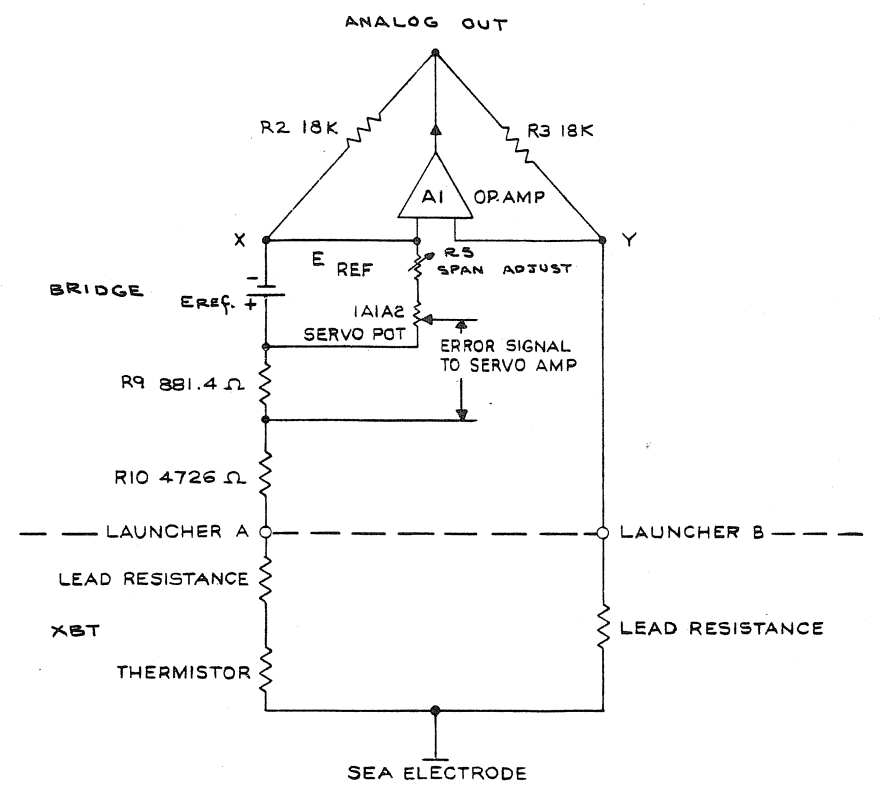
\includegraphics[width=\textwidth]{graficos/puente.png}
\caption{Circuito simplificado del puente de medici�n de la sonda XBT. Imagen tomada de \citep{sippican}}
\label{fig:puente}
\end{figure}

En el circuito de la figura \ref{fig:puente}, se utiliza un amplificador operacional para mantener la ca�da de tensi�n en cero entre los nodos X e Y y de esta manera igualar las ca�das de tensi�n en R2 y R3 y por consiguiente, igualar las corrientes en ambas ramas superiores del puente.  Dado que el amplificador operacional posee alta impedancia de entrada, virtualmente no toma corriente en su entrada y las corrientes en las ramas inferiores resultan iguales a las corrientes en las ramas superiores.  De esta manera, las corrientes en ambas ramas inferiores resultan iguales entre s�.

Cuando el sistema est� en modo medici�n (MEASSURE MODE) y la sonda est� descendiendo en el agua, el termistor se encuentra conectado a la rama inferior izquierda del puente a trav�s de la resistencia del bobinado indicada en el circuito esquem�tico como \textit{LEAD RESISTANCE}.  El otro extremo del termistor se conecta a la masa del barco a trav�s del camino conductor que forma el agua de mar entre el \textit{SEA ELECTRODE} de la sonda y el casco del barco. Las resistencias de los bobinados de ambas ramas se encuentras apareadas en un valor aproximado de 5 $k\Omega$.

Como puede verse en la figura \ref{fig:puente}, la resistencia total de la rama inferior izquierda excede a la resistencia total de la rama inferior derecha del circuito puente en una cantidad igual a la suma de $R9$, $R10$ y la resistencia del termistor, $R_{th}$.  Dado que las corrientes en ambas ramas son iguales y que las tensiones en los puntos X e Y son iguales, la suma de las ca�das de tensi�n en $R9$, $R10$ y $R_{TH}$ se debe igualar a la tensi�n de la fuente $E_{ref}$, esto es:

\begin{equation}
 I = \frac{E_{ref}}{R9 + R10 + R_{TH}} = \frac{E_{ref}}{5607,4\; \Omega + R_{TH}}
\end{equation}

\noindent donde $I$ es la corriente de la rama izquierda del puente que resulta proporcional a la temperatura que registra el termistor.

\subsection{Esquema de conexionadado}
\label{subsec:conexionado}

Un esquema de conexionado entre las tres unidades que forman el sistema de registro de trazos batitermogr�ficos Sippican se muestra en la FIG. \ref{fig:esquema-sippican}. En la figura se puede apreciar que las unidades uno (registrador MK 2A-1), dos (lanzador) y tres (sondas XBT) se conectan a trav�s de 4 se�ales: A, B, C y GND.  Cabe destacar que entre la sonda XBT y el lanzador, la se�al de GND se cierra por un camino conductor a trav�s del agua de mar, entre el \textit{sea electrode} y el casco del barco. Esto �ltimo es lo que permite identificar que la sonda ha ingresado al agua y dispara el comienzo de una medici�n de temperatura en la columna de agua.
  
\begin{figure}[htpb]
\centering
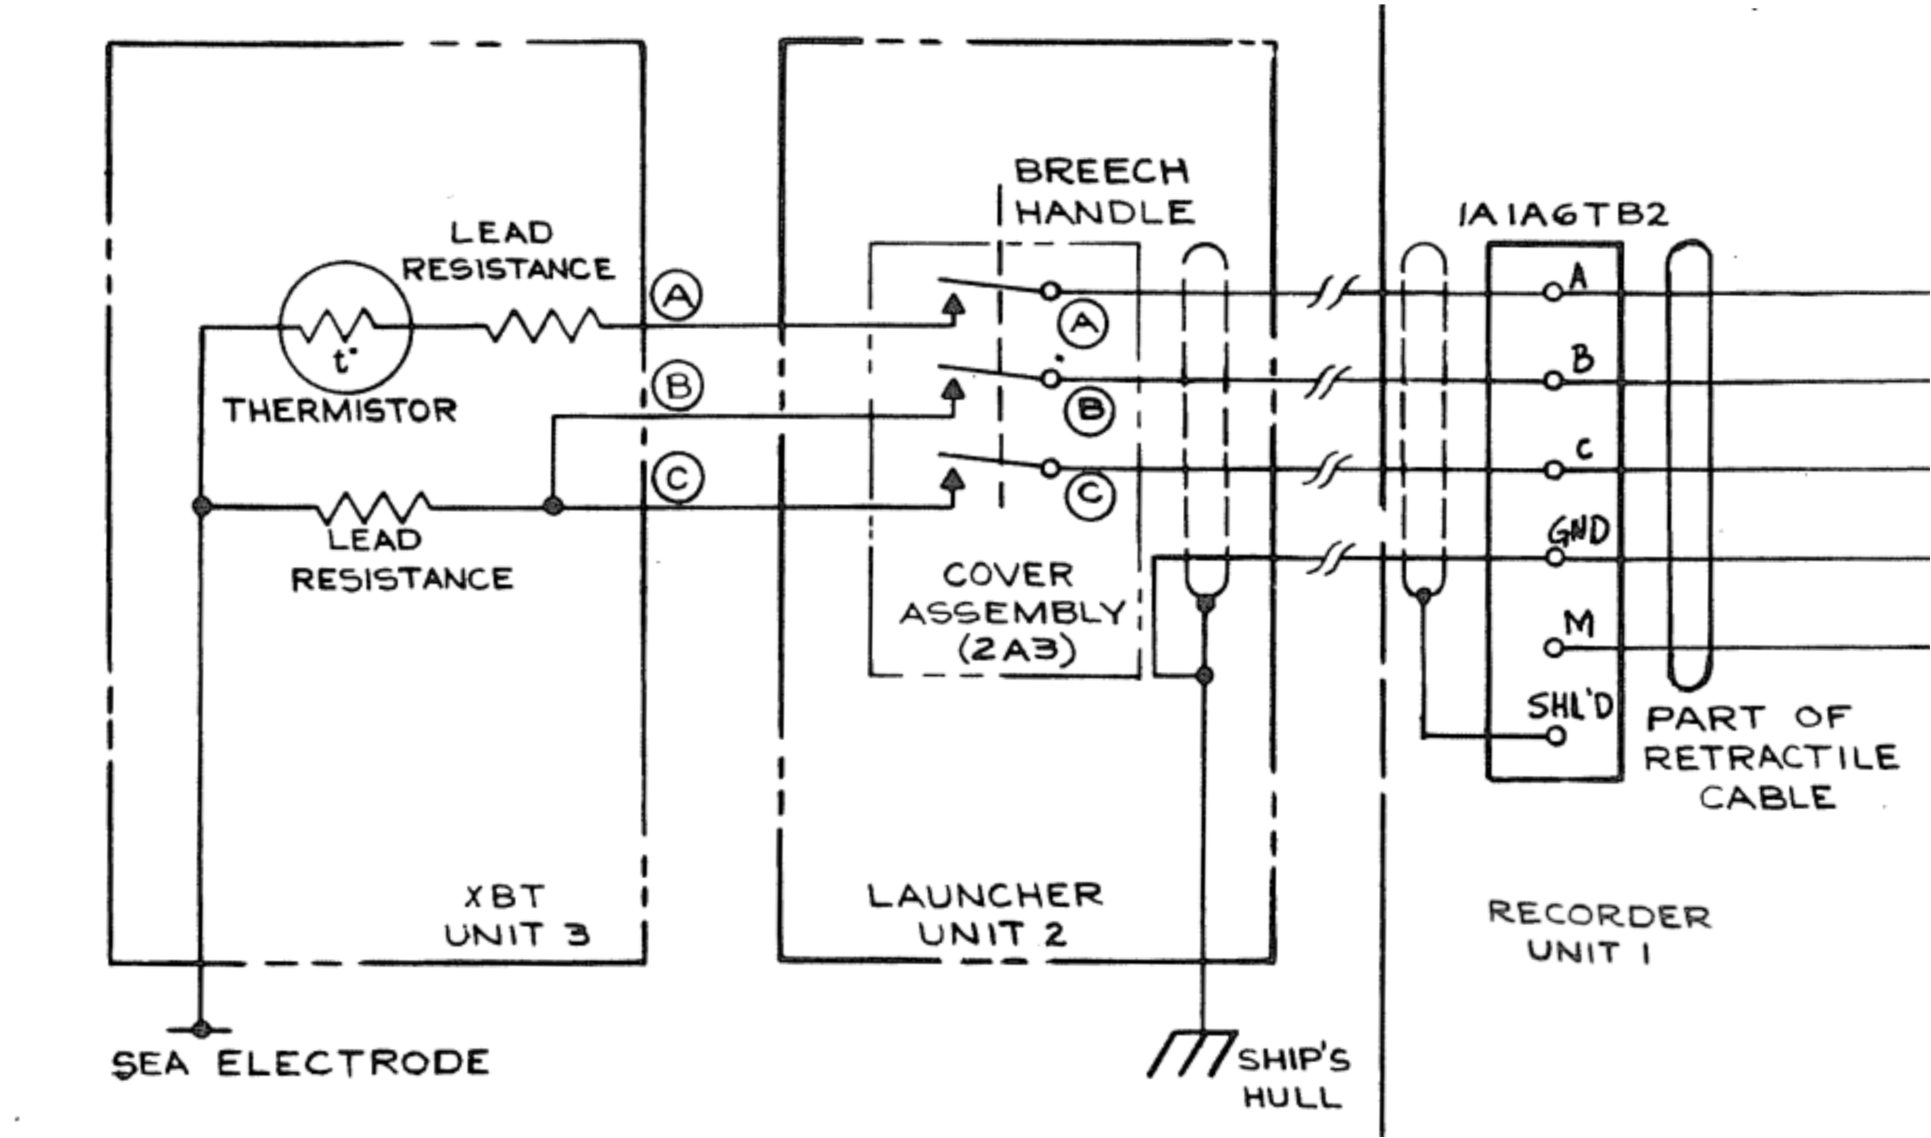
\includegraphics[width=.9\textwidth]{graficos/esquema-Sippican.pdf}
\caption{Esquema de conexionado entre las tres unidades del sistema Sippican. Imagen adaptada de \citep{sippican}}
\label{fig:esquema-sippican}
\end{figure}

En la FIG. \ref{fig:esquema-sippican} tambi�n puede apreciarse un modelo el�ctrico de la sonda XBT compuesto por los terminales A, B, C y SEA ELECTRODE, el termistor y los dos resistores asociados a los devanados que permiten independizar el desplazamiento del buque del descenso de la sonda.

La bornera 1A1A6TB2 se encuentra accesible a trav�s de un panel desmontable sobre el lateral izquierdo del registrador, como puede apreciarse en la FIG. \ref{fig:panel-lateral}.  A esta bornera llevan las cuatro se�ales provenientes del lanzador, A, B, C y GND.

\begin{figure}[htpb]
\centering
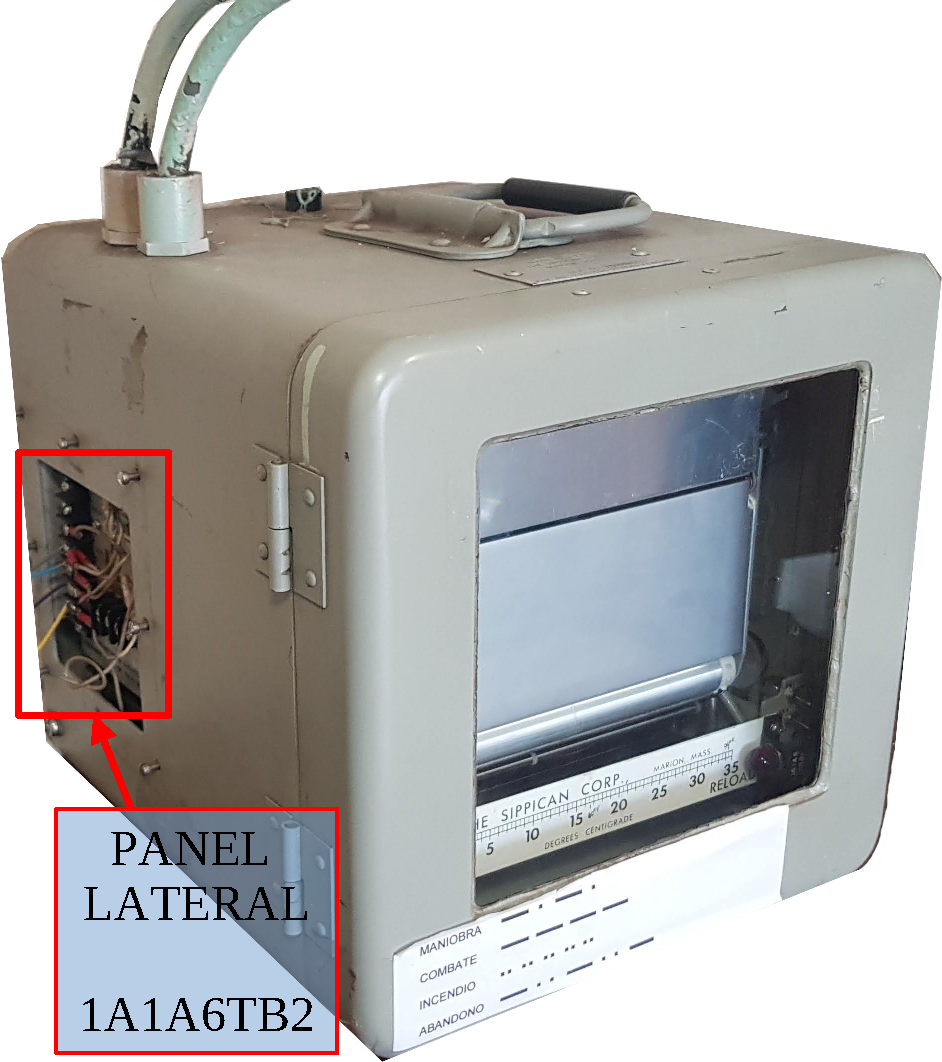
\includegraphics[width=.4\textwidth]{graficos/panel-lateral.pdf}
\caption{Ubicaci�n del panel lateral de acceso a la bornera 1A1A6TB2 del registrador MK 2A-1}
\label{fig:panel-lateral}
\end{figure}

\section{SONDA BATITERMOGR�FICA DESCARTABLE}
\label{sec:sonda}

Los batiterm�grafos descartables, referidos com�nmente como XBTs est�n compuestos por una sonda con forma bal�stica, un c�nister, una bobina de cable dentro del c�nister, un pin de lanzamiento y una tapa de cierre protectora para su almacenamiento.  El pin de lanzamiento retiene la sonda dentro del c�nister y cuando se saca, la sonda cae al agua por efecto de la gravedad. La sonda contiene un termistor, que es el elemento sensible a la temperatura y que se encuentra conectado a una bobina de cable dentro de la sonda.  El otro extremo del cable est� enrollado a una segunda bobina dentro del c�nister.  La t�cnica de doble bobina permite que el cable quede libre en el agua en el punto de entrada y no se vea afectado por el movimiento del barco ni el descenso de la sonda.

En la figura \ref{fig:probe} se puede observar, a la izquierda, una vista de despiece con los componentes del batiterm�grafo junto con una fotograf�a de un XBT real dentro de su c�nister a la derecha.


\begin{figure}[htpb]
\centering
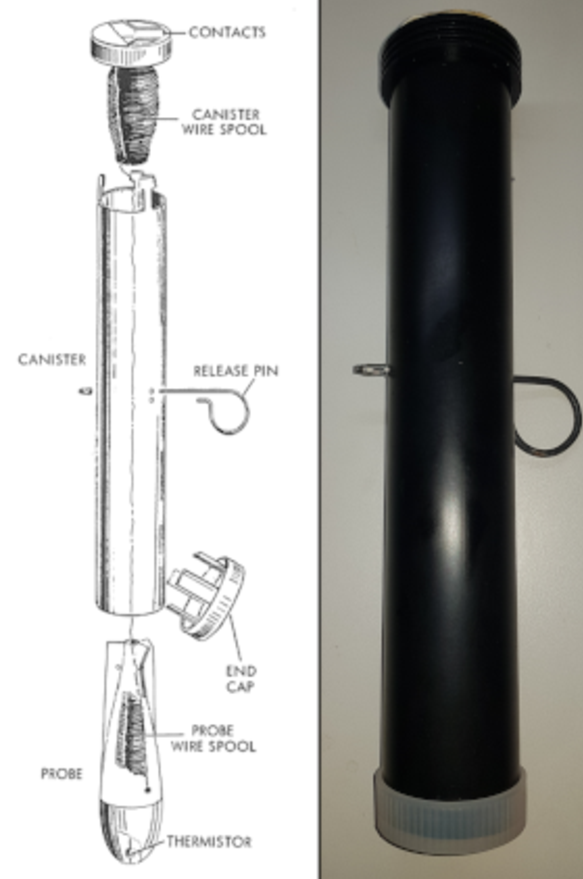
\includegraphics[width=.6\textwidth]{graficos/ProbeXBT.pdf}
\caption{\underline{Izquierda:} vista de los componentes de un XBT, figura tomada del manual \citep{sippican}. \underline{Derecha:} foto de un XBT real.}
\label{fig:probe}
\end{figure}

Las sondas se clasifican por su m�xima profundidad alcanzable y la m�xima velocidad de operaci�n del buque del cual son lanzadas:

\begin{itemize}
\item T-4: XBT 1500 pies, 30 nudos.
\item T-5: XBT 6000 pies, 6 nudos.  Requiere un accesorio para el registrador, KOR-6.
\item T-6: XBT 1500 pies, 13 nudos.
\item T-7: XBT 2500 pies, 15 nudos. Requiere un accesorio para el registrador, KOR-6.
\item T-10: XBT 660 pies, 10 nudos. Requiere un accesorio para el registrador, KOR-12.
\item T-11: FSXBT 1560 pies, 6 nudos. Requiere un accesorio para el registrador, KOR-6.
\end{itemize}

%A su vez, las distintas sondas XBT pueden requerir distintos tipo de rollos de papel para el registrador.
Las sondas T-4, T-6 y T-7 tienen la misma masa, las mismas caracter�sticas hidrodin�micas y la misma ecuaci�n para el c�lculo de la profundidad en funci�n del tiempo. Las sondas T-5 y T-11 tienen diferente masa, caracter�sticas hidrodin�micas y ecuaci�n de profundidad en funci�n del tiempo.  En la tabla \ref{tabla:sondas} se reunen las ecuaciones emp�ricas de profundidad vs. tiempo en unidades m�tricas est�ndar junto con las profundidades m�ximas alcanzables y el tiempo que le insume a la sonda llegar a esa profundidad.

\begin{table}[htpb]
\centering
\caption{Ecuaciones emp�ricas de profundidad vs tiempo de entrada para los distintos tipos de sondas.}
\label{tabla:sondas}
\begin{tabular}{c|c|c|c}
Tipo & Prof H(m) vs tiempo t(s) & M�xima profundidad (m) & Tiempo para m�x prof. (s) \\ \hline
T-10		& $H = 6,301\cdot t - 0,00216\cdot t^2$ & 200	& 32,4 \\
T-4, T-6	& $H = 6,472\cdot t - 0,00216\cdot t^2$ & 460	& 72,9 \\
T-7			& $H = 6,472\cdot t - 0,00216\cdot t^2$ & 760	& 122,4 \\
T-5			& $H = 6,828\cdot t - 0,00182\cdot t^2$ & 1830	& 290,6 \\
T-11		& $H = 1,7779\cdot t - 0,000255\cdot t^2$ & 460	& 232,3 \\
\end{tabular}
\end{table}

%\vspace{1cm}
%
%
%\vspace{1cm}

La sonda XBT posee un termistor tipo NTC (\textit{Negative Temperature Coefficient}). El valor de resistencia del termistor disminuye a medida que la temperatura asciende y se observa un comportamiento cuasi inversamente proporcional a la suma de $R_{TH}$ y 5607,4 $\Omega$. El fabricante indica la transferencia del termistor presente en las sondas XBT a trav�s de un conjunto de pares temperatura-resistencia que se muestran en la tabla \ref{tabla:transferencia}.

\begin{table}[htpb]
\centering
\caption{Transferencia del termistor presente en las sondas XBT. Pares temperatura vs. resistencia informados por el fabricante.}
\label{tabla:transferencia}
\begin{tabular}{c|c}
Temperatura (�C) & Resistencia del termistor ($\Omega$) \\ \hline
-2,0             & 18094                                \\
-1,11            & 17287                                \\
0,0              & 16329                                \\
5,0              & 12687                                \\
10,0             & 9948                                 \\
16,66            & 7274                                 \\
20,0             & 6247                                 \\
25,0             & 5000                                 \\
30,0             & 4024                                 \\
34,44            & 3350                                 \\
35,55            & 3193                                
\end{tabular}
\end{table}

A partir de la tabla \ref{tabla:transferencia} se grafica la transferencia del elemento sensor presente en las sondas XBT.  En la figura \ref{fig:transferenciaXBT} se muestra la curva de temperatura vs. resistencia del termistor. Los puntos de color rojo corresponden a lo informado por el fabricante.  La curva de color azul es una interpolaci�n polin�mica de grado 3 obtenida con el programa para realizar c�lculos num�ricos GNU Octave, cuya ecuaci�n es:

\begin{equation}
p(t) = -0,18416 \cdot t^3 + 18,96982 \cdot t^2  - 812,63985 \cdot t  + 16356,21147
\end{equation}


\begin{figure}[htpb]
\centering
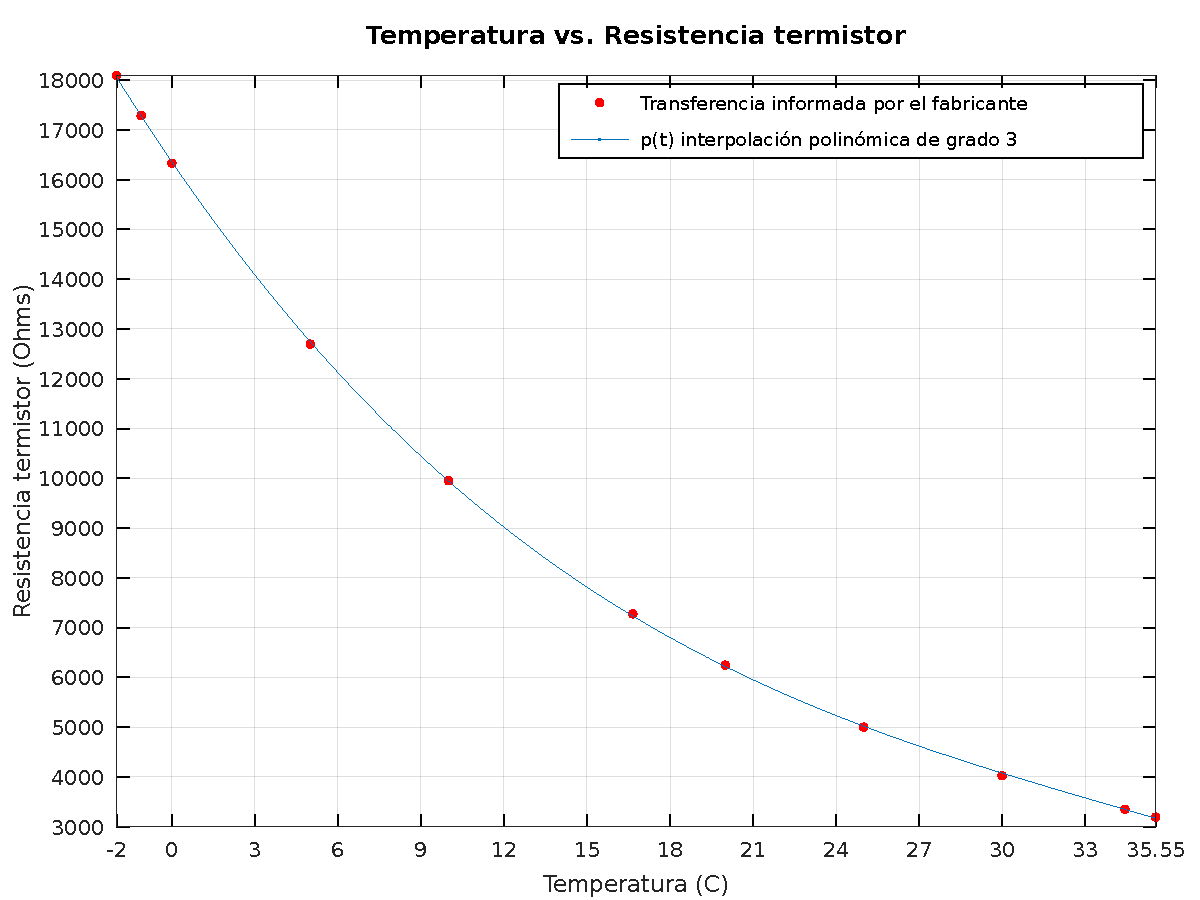
\includegraphics[width=.75\textwidth]{graficos/Temp_vs_Resistencia.pdf}
\caption{Curva de temperatura vs resistencia del termistor presente en las sondas XBT. En rojo, la transferencia informada por el fabricante. En color azul, un ajuste polin�mico de grado 3.}
\label{fig:transferenciaXBT}
\end{figure}

El circuito equivalente el�ctrico de la sonda XBT que forma parte de la FIG. \ref{fig:esquema-sippican}, se repite separado en la FIG. \ref{fig:equivalenteXBT} para mayor claridad. En esta figura se puede apreciar al termistor o elemento que mide la temperatura modelado como un resistor junto con otros dos resistores, indicados como \textit{LEAD RESISTANCE}, que modelan el efecto resistivo de los hilos conductores que conectan el termistor con la embarcaci�n.  Tambi�n se pueden ver los cuatro terminales, A, B, C y \textit{SEA ELECTRODE} que constituyen la interfaz de la sonda. 

El termistor se conecta con dos hilos conductores que se encuentran unidos solidarios, recubiertos con una pintura tipo barniz para garantizar la aislaci�n el�ctrica y bobinados en dos arrollamientos, uno dentro de la sonda con forma bal�stica que desciende por la columna de agua y otro en el c�nister que permanece dentro del lanzador que se mueve solidario a la embarcaci�n.  De esta manera, cada \textit{LEAD RESISTANCE} representa el valor resistivo total de un hilo conductor que se encuentra arrollado mitad en la bobina dentro de c�nister y mitad dentro de la bobina dentro de la sonda.  Esto le permite al fabricante de las sondas garantizar que estos valores resistivos est�n precisamente apareados, debido a que surgen de conductores con id�ntica conductividad, secci�n y longitud.

Un extremo del termistor se conecta a trav�s de uno de los hilos conductores con el terminal A y a trav�s del otro hilo conductor con los terminales B y C.  Este �ltimo extremo tambi�n est� expuesto al agua de mar en un contacto indicado como \textit{SEA ELECTRODE} que permite cerrar una camino conductor con el casco de la embarcaci�n a trav�s del agua de mar y que se utiliza para detectar el lanzamiento de la sonda y su ingreso al agua.

 
%Por otra parte, los terminales B y C se conectan al resistor indicado en la FIG. \ref{fig:equivalenteXBT} tambi�n como \textit{LEAD RESISTANCE}, que modela el devanando o arrollamiento de cable en la bobina que se encuentra dentro del c�nister.  Este devanado se queda en el lanzador y se desplaza solidario con la embarcaci�n.
 
El fabricante de las sondas garantiza que los valores de resistencia de cada par de \textit{LEAD RESISTANCE} est�n apareados en un valor cercano a los 5 K$\Omega$ para cada sonda.  Ensayos preliminares sobre sondas tipo \text{T-6} y {T-7} mostraron que los valores de resistencia de las \textit{LEAD RESISTANCE} pueden variar conjuntamente seg�n el tipo de sonda. Esto resulta esperable, debido a que los respectivos devanados tienen distinta cantidad de metros de cable, funci�n de la profundidad m�xima alcanzable por cada tipo sonda.  

Desde el punto de vista de la sonda, los terminales B y C se encuentran siempre cortocircuitados.  Esto permite que desde el lanzador se detecte la presencia de una sonda lista para ser lanzada a trav�s de la presencia o no de este cortocircuito
%
%La variabilidad de las \textit{LEAD RESISTANCE} hace que sea conveniente medir la temperatura de forma diferencial a fin de descartar las contribuciones de estas resistencias 



\begin{figure}[htpb]
\centering
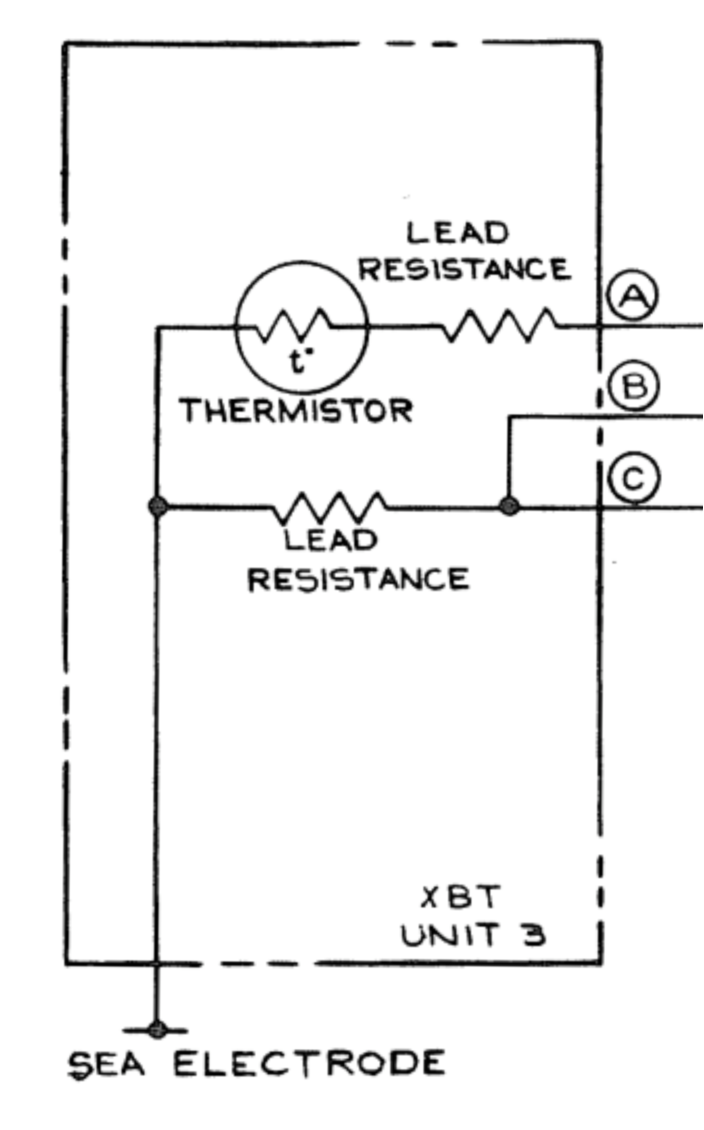
\includegraphics[width=.3\textwidth]{graficos/equivalenteXBT.pdf}
\caption{Circuito el�ctrico equivalente de una sonda XBT.}
\label{fig:equivalenteXBT}
\end{figure}

\section{DISE�O CIRCUITAL}
\label{sec:dise�o}

Se consideraron distintas alternativas para el dise�o de la interfaz circuital o etapa de acondicionamiento de las se�ales de las sonda XBT. Una primera caracter�stica a definir fue si se iba a reemplazar el sistema de registro Sippican o no ya que el dise�o el�ctrico de la interfaz depende fuertemente de esta caracter�stica. La lectura del valor de temperatura del XBT depende de que se energice la sonda externamente, debido a las sonda XBT son pasivas. Si se opta por reemplazar al sistema de registro Sippican, la interfaz que se dise�e debe proveer un mecan�smo para excitar al termistor presente en la sonda.  Cabe aclarar que la excitaci�n de la sonda es una funci�n excluyente de uno u otro componente y que no puede ser realizada por ambos en simult�neo.

La etapa de acondicionamiento o interfaz circuital act�a como enlace entre la sonda XBT y una etapa de digitalizaci�n que se implementa con un kit de desarrollo NUCLEO-STM32F429ZI, basado en un microcontrolador Cortex-M4 de STMicroelectronics.  Por este motivo, los niveles de tensi�n de salida de la interfaz se deben mantener en el rango 0-3,3 V para evitar posibles da�os en las entradas de los conversores anal�gicos digitales del kit.  

Por un lado, se exploraron circuitos que funcionan en conjunto con el registrador Sippican sin afectar su operaci�n.  Estas interfaces deber�an permitir hacer lecturas de tensi�n del circuito puente de la FIG. \ref{fig:puente}, para obtener un valor de tensi�n proporcional a la ca�da de tensi�n sobre el termistor.  Se ensayaron circuitos con amplificadores operaciones basado en la configuraci�n de amplificador diferencial, en particular con dos topolog�as circuitales, una conocida como \textit{scaling-substractor} o escalador-restador y otra como amplificador diferencial con \textit{buffers} de entrada. 

Por otra parte, se dise�� un circuito en base a dos fuentes de corriente que reemplaza al registrador Sippican. Esta interfaz permite hacer lecturas de tensi�n y, en forma indirecta, de corriente para poder calcular el valor de resistencia del termistor de la sonda XBT.  Asimismo, como esta interfaz reemplaza el sistema de registro Sippican, se contempla la captura de los distintos modos de funcionamiento  \textit{reload, launch, meassure} para no modificar los procedimiento de operaci�n conocidos por los usuarios operativos navales, para los que el cambio de un sistema a otro deber�a ser ``transparente''.

Finalmente, se consider� un dise�o disponible en la literatura \citep{STEGEN1975447}. Se trata de un circuito puente balanceado que utiliza un transistor de efecto de campo JFET para ``copiar'' el valor resistivo del termistor de la sonda.  Esta interfaz reemplaza al registrador Sippican.

En las siguientes subsecciones se abordan los detalles de dise�o.% y se realiza una comparativa de los tres enfoques considerados. 

\clearpage

\subsection{Dise�os que funcionan en conjunto con el registrador Sippican}

\subsubsection{Scaling-substractor}

El primer dise�o considerado para funcionar en conjunto con el registrador Sippican se basa en la topolog�a \textit{scaling-substractor}.  Este dise�o se basa en un amplificador operacional realimentado, funcionando como amplificador diferencial. En la FIG. \ref{fig:opAmp_diferencial} se muestra un esquema de amplificador diferencial que sirve para calcular su transferencia.

\begin{figure}[htpb]
\centering
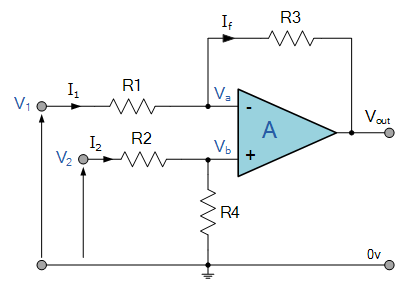
\includegraphics[width=.55\textwidth]{graficos/opAmp_diferencial.png}
\caption{Circuito el�ctrico de un amplificador diferencial.}
\label{fig:opAmp_diferencial}
\end{figure}

Se puede deducir que la salida $V_{out}$ del circuito en funci�n de las entradas $V_1$ y $V_2$ es:

\begin{equation}
V_{out} = -V1 \cdot \left(\frac{R_3}{R_1}\right) + V_2 \cdot \left(\frac{R_4}{R_2 + R_4}\right) \cdot \left(\frac{R_1 + R_3}{R_1}\right)
\end{equation}

\noindent cuando se hace $R_1 = R_2$ y $R_3 = R_4$, se puede simplificar la expresi�n a: 

\begin{equation}
V_{out} = \left(\frac{R_3}{R_1}\right) \cdot \left(V_2 - V_1\right)
\label{ec:opamp}
\end{equation}

\noindent donde se aprecian la naturaleza de la resta de tensi�n que realiza el circuito entre sus entradas $V_1$ y $V_2$ y el factor de escala $\left(\frac{R_3}{R_1}\right)$ que dan nombre a esta topolog�a circuital \citep{rashid1999circuitos}.

Se ensay� un dise�o que toma la tensi�n del terminal B de la sonda.  Esto resulta muy conveniente debido a que se puede utilizar directamente la bornera 1A1A6TB2, que se encuentra accesible a trav�s de un panel desmontable sobre el lateral izquierdo del registrador Sippican.

Este dise�o agrega al amplificador diferencial un segundo amplificador operacional en configuraci�n seguidor por emisor para evitar efectos de carga sobre el puente balanceado Sippican. Asimismo, se agreg� un divisor resistivo conectado a la entrada inversora para controlar la tensi�n que se resta y ajustar el cero de la salida $V_{out}$.  Los valores de $R_1$ y $R_3$ se ajustan para que la salida no sature.

Se eligi� un amplificador operacional de tipo \textit{rail to rail} con el objetivo de que la excursi�n de la salida pueda variar en todo el rango de tensi�n desde 0 V hasta la tensi�n de alimentaci�n, elegida en +3,3 V para que sea compatible con los niveles de tensi�n de las entradas del ADC de la placa NUCLEO-STM32F429ZI. 

Por otra parte, los amplificadores operacionales utilizan alimentaci�n simple de +3,3 V, en lugar de alimentaci�n doble, con tensi�n positiva y negativa.  Esto simplifica en gran medida el dise�o y reduce el conteo de componente, lo que hace m�s conveniente el dise�o que puede alimentarse incluso de la propia placa NUCLEO-STM32F4ZI.

En la FIG. \ref{fig:scaling} se muestra el circuito puente simplificado del registrador Sippican con circuito interfaz \textit{scaling substractor} conectado en el punto indicado como Launcher\_B.  Se observan dos amplificadores operaciones en configuraci�n seguidor por emisor y amplificador diferencial, respectivamente.  En el circuito se puede apreciar que se utiliza la aproximaci�n polin�mica de la transferencia del termistor para realizar un barrido param�trico en todo el rango de temperatura, desde -2,0 �C a 35,5 �C.

\begin{figure}[htpb]
\centering
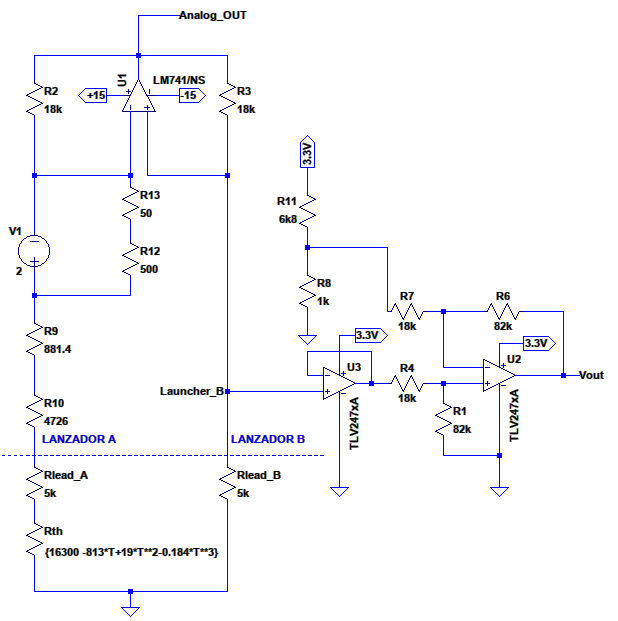
\includegraphics[width=.98\textwidth]{graficos/scaling_circuito.png}
\caption{Circuito el�ctrico esquem�tico de la interfaz \textit{scaling-substractor}.}
\label{fig:scaling}
\end{figure}

En la FIG. \ref{fig:salida_scaling} se muestra la salida de tensi�n del \textit{scaling substractor}, $V_{out}$ para dos conjuntos alternativos de valores de resistores. Se grafica la salida $V_{out}$  en funci�n de la temperatura para todo el rango de operaci�n de las sondas XBT, desde -2,0 �C a 35,5 �C.  Para esto se utiliz� el polinomio interpolador descripto en la secci�n \ref{sec:sonda} que modela la transferencia del termistor.

Existe una relaci�n de compromiso entre la linealidad de $V_{out}$ y su rango din�mico. Cabe notar, en la FIG. \ref{fig:salida_scaling}, un leve efecto de alinealidad entre -2,0 �C y -1,0 �C para el trazo azul, que puede corregirse reduciendo el rango din�mico de $V_{out}$. Por ejemplo, se puede aumentar el valor de R11 a 8k2 $\Omega$ y aumentar los valores de R4 y R7 a 22 $k\Omega$.  Esto producir�a una salida m�s lineal pero con menor rango din�mico como puede verse en el trazo rojo de la misma figura. 

\begin{figure}[htpb]
\centering
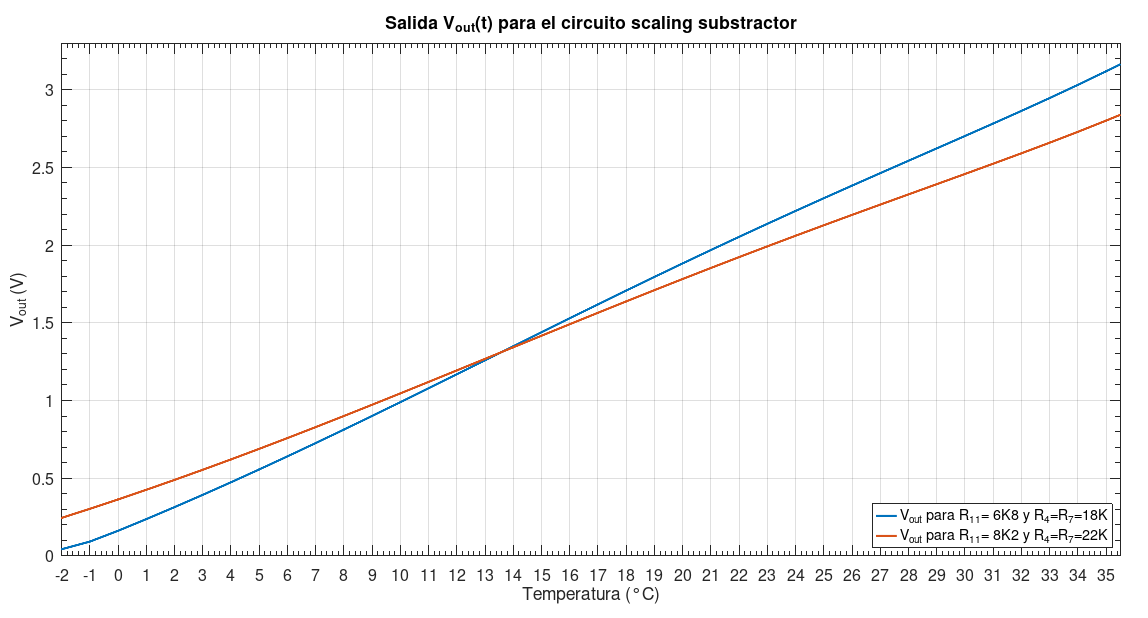
\includegraphics[width=.92\textwidth]{graficos/scaling_Vout(t).png}
\caption{Vout para dos conjuntos alternativos de valores de resistores. En trazo azul, $R_{11}= 6K8\; \Omega \text{ y } R_4=R_7=18 \; K\Omega$. En trazo rojo, $R_{11}\;= 8K2\; \Omega \text{ y } R_4=R_7=22\; K\Omega$.}
\label{fig:salida_scaling}
\end{figure}

El dise�o del circuito acondicionador \textit{scaling substractor} tiene un problema inherente a la forma en que toma la se�al del puente Sippican, en un �nico punto, directamente del terminal B.  Si bien en principio esta parec�a ser una ventaja, por la simplicidad del dise�o, se encontr� que esta configuraci�n es sensible a la variabilidad en el valor de $R_{lead}$ que hay entre los diferentes tipos de sondas, por lo que resulta inadecuado para la aplicaci�n. En la FIG. \ref{fig:scaling_vs_Rlead} se muestra la familia de curvas de salida del circuito \textit{scaling substractor}, $V_{out}$, para diferentes valores de $R_{lead}$ entre 4K7 y 8K2 $\Omega$.

\begin{figure}[htpb]
\centering
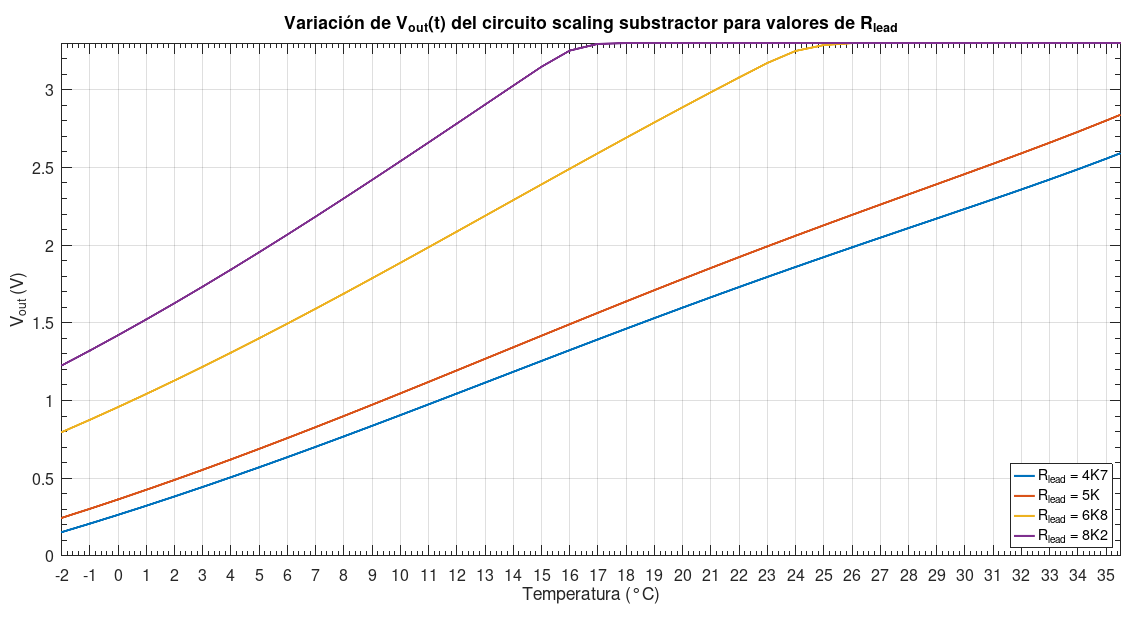
\includegraphics[width=.92\textwidth]{graficos/scaling_Vout_vs_Rlead.png}
\caption{Familia de curvas Vout para diferentes valores de $R_{lead}$.}
\label{fig:scaling_vs_Rlead}
\end{figure}

\subsubsection{Amplificador diferencial con \textit{buffers} de entrada}
\label{subsubsec:ampDiferencial}

El segundo dise�o considerado para funcionar en conjunto con el registrador Sippican trabaja en modo diferencial, es decir, tomando dos se�ales del puente Sippican en lugar de solo una. Esta caracter�stica lo hace particularmente adecuado para descartar las contribuciones de las $R_{lead}$ y superar las limitaciones del dise�o basado en el \textit{scaling-substractor} antes mencionadas.  Asimismo, incorpora un segundo \textit{buffer} de entrada para desacoplar impedancias.

%Este dise�o consta de dos \textit{buffers} o seguidores por emisor para desacoplar impedancias y no cargar el circuito puente del registrador Sippican, de donde se toman las se�ales. 

%El \textit{quid} de la cuesti�n es identificar de qu� dos puntos tomar la 

En la FIG. \ref{fig:opAmp_diferencial_2} se muestra un esquema de la topolog�a utilizada. La salida $V_{out}$ en funci�n de $V_1$ y $V_2$ es la misma que fue presentada en la EC. \ref{ec:opamp}. En este caso, no se utiliza una entrada con tensi�n fija para $V_1$, como en el primer dise�o, sino que esta se conecta directamente a otro punto del puente Sippican.

\begin{figure}[htpb]
\centering
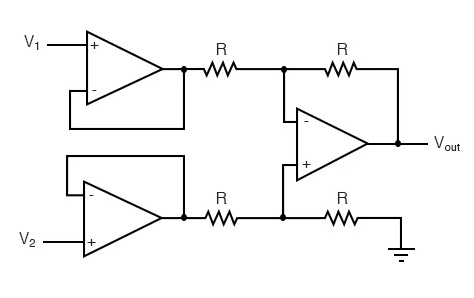
\includegraphics[width=.45\textwidth]{graficos/opAmp_diferencial_2.png}
\caption{Circuito el�ctrico de un amplificador diferencial con \textit{buffers} de entrada.}
\label{fig:opAmp_diferencial_2}
\end{figure}

Para el caso particular de $R_1 = R_2 = R_3 = R_4 = R$, la expresi�n de $V_{out}$ de la EC.\ref{ec:opamp} se puede simplificar para obtener la expresi�n del amplificador diferencial con ganancia unitaria:

\begin{equation}
V_{out} = \left(V_2 - V_1\right)
\end{equation}

Este dise�o toma dos se�ales del registrador Sippican, Analog\_OUT y Launcher\_A. El acceso a Analog\_OUT no es directo y requiere de una conexi�n al pin r de la bornera 1A1A6J1 disponible en la parte trasera interna del registrador MK 2A-1, como se muestra en la FIG. \ref{fig:bornera_1A1A6J1}.  

\begin{figure}[htpb]
\centering
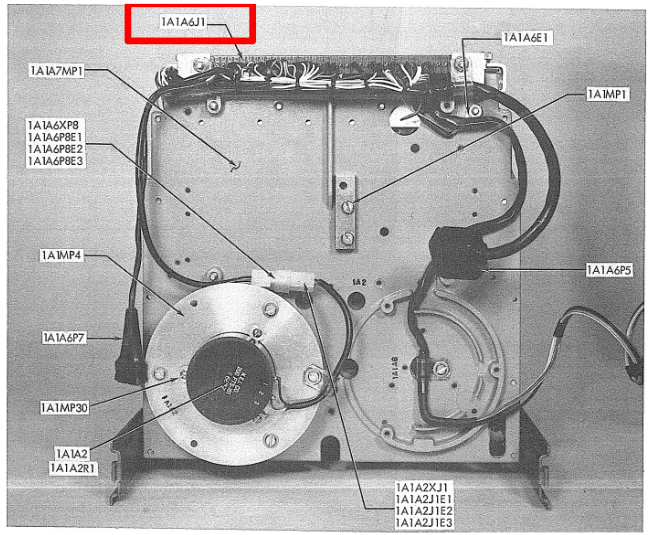
\includegraphics[width=.6\textwidth]{graficos/bornera_1A1A6J1.png}
\caption{Ubicaci�n de la bornera 1A1A6J1 para acceso a la se�al Analog\_OUT del puente Sippican.}
\label{fig:bornera_1A1A6J1}
\end{figure}

Por otra parte, Analog\_OUT se encuentra disponible en la bornera 1A1A6TB2, de f�cil acceso a trav�s de un panel desmontable del registrador, como fuera mostrado en la FIG. \ref{fig:panel-lateral}.

Este dise�o, si bien es funcional y resuelve la dependencia con $R_{lead}$ que tiene la topolog�a \textit{scaling-substractor}, incorpora la necesidad de utilizar fuente de alimentaci�n doble $\pm 15$V para todos los amplificadores operacionales a fin de lograr la excursi�n deseada para la se�al de salida.  Esta caracter�stica agrega complejidad al dise�o que ya no podr� alimentarse de la placa NUCLEO-STM32F429ZI sino que requerir� una fuente de alimentaci�n propia e independiente.

En la FIG. \ref{fig:ampliDiferencial} se puede observar el circuito esquem�tico propuesto junto con el puente Sippican simplificado.  Cabe observar que las entradas del amplificador diferencial se toman de los puntos indicados como Launcher\_A y Analog\_OUT. 

\vspace{10px}
\begin{figure}[htpb]
\centering
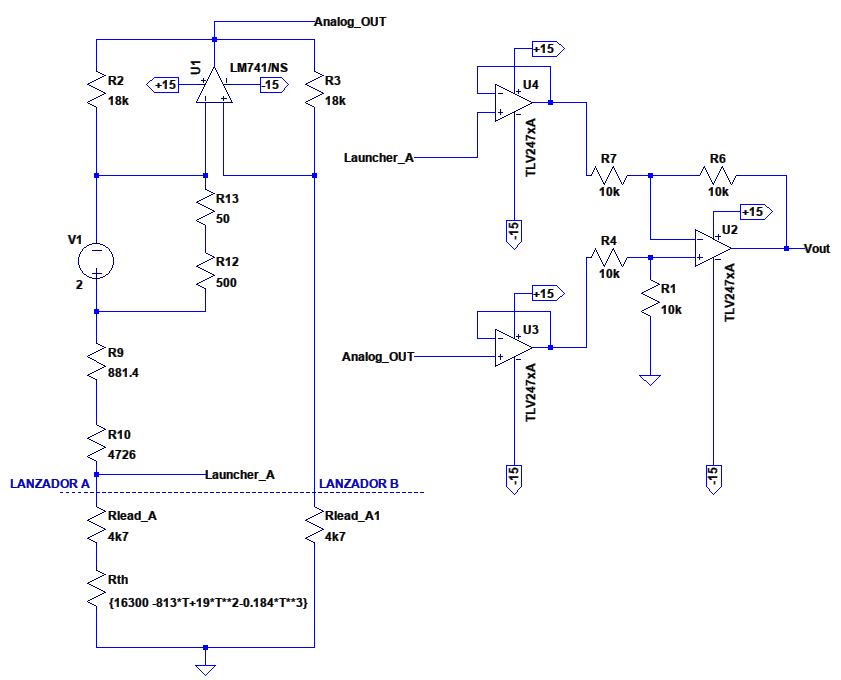
\includegraphics[width=1\textwidth]{graficos/disenio2_circuito.png}
\caption{Circuito el�ctrico esquem�tico de la interfaz con un amplificador diferencial con \textit{buffers} de entrada.}
\label{fig:ampliDiferencial}
\end{figure} 
\vspace{20px}

En el circuito se puede apreciar que se utiliza la misma aproximaci�n polin�mica presentada en la secci�n \ref{sec:sonda} para modelar la transferencia del termistor.  Con esta aproximaci�n se puede analizar el comportamiento del circuito dise�ado para cualquier valor de temperatura directamente sin tener que recurrir a una tabla con los pares de valores puntuales que ofrece el fabricante.

La tensi�n de salida $V_{out}$ crece linealmente con la temperatura en todo el rango desde -2,0 �C a 35,5 �C, como se puede observar en la simulaci�n param�trica de la FIG.\ref{fig:salida_ampDiff}.

\begin{figure}[htpb]
\centering
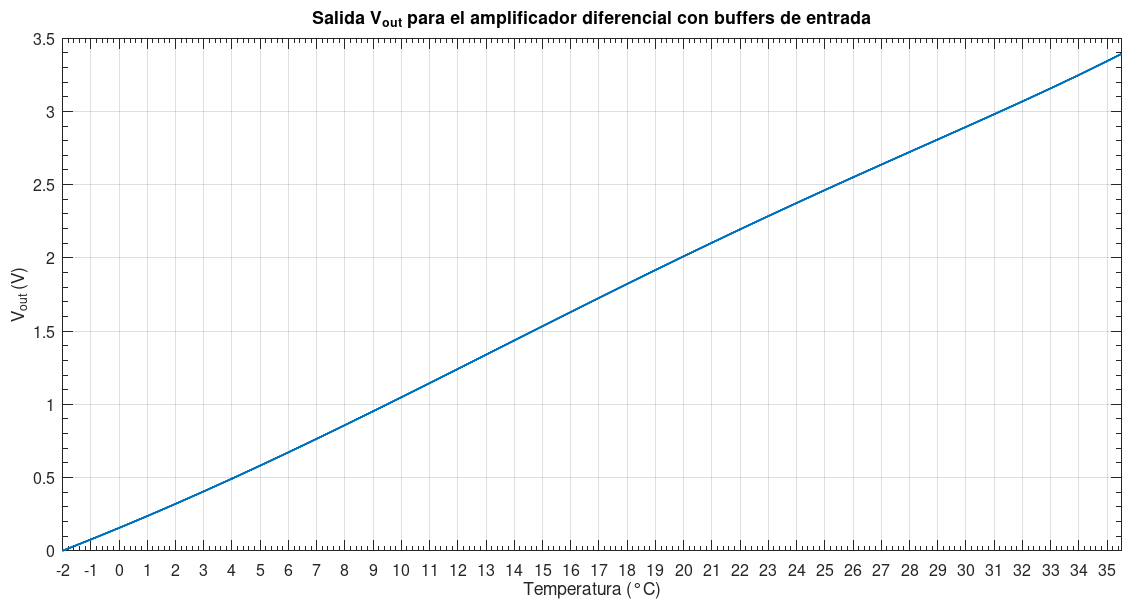
\includegraphics[width=.98\textwidth]{graficos/disenio2_Vout.png}
\caption{Vout para el segundo dise�o basado en un amplificador diferencial con \textit{buffers} de entrada.}
\label{fig:salida_ampDiff}
\end{figure}

Por otra parte, se analiza en la FIG.\ref{fig:ampDiff_vs_Rlead}, la dependiencia de $V_{out}$ con $R_{lead}$ para cuatro valores discretos de resistencia: 4k7 $\Omega$, 5K $\Omega$, 6k8 $\Omega$ y 8k2 $\Omega$ variados de a pares, es decir que ambos $R_{lead}$ tienen el mismo valor para cada paso de la simulaci�n. Las cuatro curvas de la familia son coincidentes por lo que se concluye que no hay dependencia.

\begin{figure}[htpb]
\centering
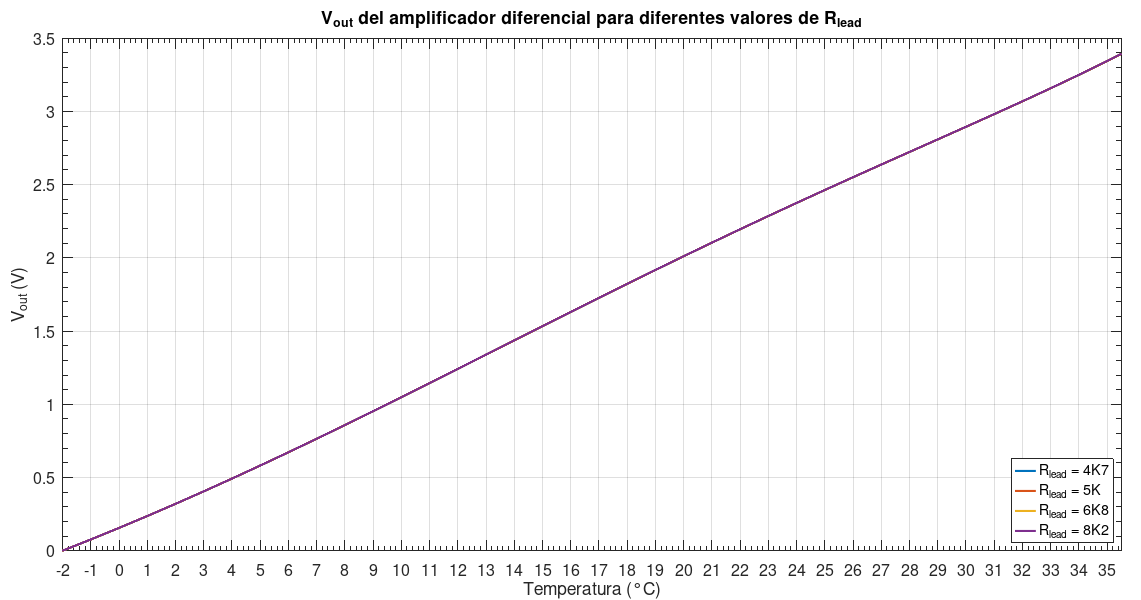
\includegraphics[width=.98\textwidth]{graficos/disenio2_Vout_vs_Rlead.png}
\caption{Familia de curvas Vout para diferentes valores de $R_{lead}$.}
\label{fig:ampDiff_vs_Rlead}
\end{figure}

\clearpage

\subsection{Dise�o con dos fuentes de corriente}
\label{subsec:2fuentes}

A partir del concepto general del dise�o incorporado en el registrador Sippican y del dise�o del puente balanceado, se desarroll� un circuito auxiliar que permite realizar directamente la medici�n de temperatura de la sonda XBT. Este dise�o reemplaza al registrador Sippican y no puede funcionar en conjunto con �l debido a que tambi�n provee alimentaci�n a la sonda XBT, y esta caracter�stica los hace mutuamente excluyentes.

Se propuso obtener una tensi�n proporcional al valor resistencia del termistor, dentro del rango 0 V - 3,3 V.  Este rango de tensi�n es compatible con el rango de las entradas anal�gicas de la mayor�a de los microcontroladores y conversores anal�gico-digitales. El circuito consiste en dos fuentes de corriente que operan de manera independiente y alimentan cada rama del circuito de la sonda XBT. La FIG. \ref{fig_principio_funcionamiento} muestra el principio de funcionamiento. 

\vspace{10px}
\begin{figure}[htpb]
	\centering
	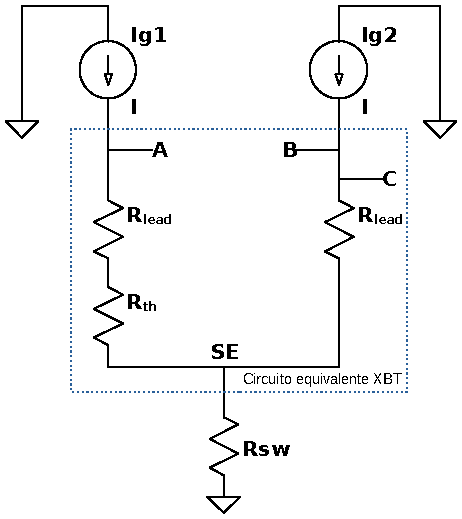
\includegraphics[width=0.5\textwidth]{graficos/Principio_funcionamiento.pdf}
	\caption{Principio de funcionamiento del dise�o con dos fuentes de corriente.}
	\label{fig_principio_funcionamiento}
\end{figure}
\vspace{10px}
Las fuentes $I_\text{g1}$ e $I_\text{g2}$ entregan corrientes id�nticas de magnitud $I$. Si el XBT est� en modo \textit{measure}, lo que implica que est� desplegado en la columna de agua, el nodo SE (en ingl�s, \textit{Sea Electrode}) est� inmerso en agua de mar y, por lo tanto, est� vinculado a la tierra de la embarcaci�n a trav�s de la resistencia del agua, $R_\text{SW}$. Las resistencias $R_\text{lead}$ representan los devanados del XBT y $R_\text{th}$ es la resistencia del termistor. 

La existencia de una tensi�n no nula entre los puntos A y B , o entre A y C, es consecuencia de la ca�da de potencial en $R_\text{th}$. Dado que $I$ es conocida, el valor de $R_\text{th}$ puede obtenerse mediante la expresi�n:

\begin{equation}
R_{th} = \frac{V_\text{AB}}{I}
\end{equation}    

Las fuentes de corriente se dise�aron utilizando dos transistores bipolares PNP con resistencia de emisor y provistos de una tensi�n conocida en la base, tal como se observa en la representaci�n de la FIG. \ref{fig_disenio_definitivo_preliminar}.

\begin{figure}[htpb]
	\centering
	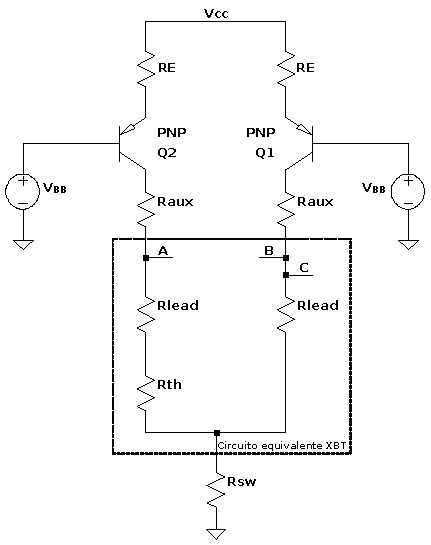
\includegraphics[width=0.7\textwidth]{graficos/Disenio_definitivo_preliminar.pdf}
	\caption{Implementaci�n de las fuentes de corriente con transistores PNP con resistencia de emisor y tensi�n conocida en la base.}
	\label{fig_disenio_definitivo_preliminar}
\end{figure}

La corriente a trav�s de cada colector, asumiendo que ambos transistores est�n en modo activo directo (MAD), est� dada por la siguiente ecuaci�n, que utiliza la nomenclatura tradicional de circuitos con transistores \citep{gray2009analysis}:

\begin{equation}
I_c = \frac{\beta}{\beta+1} \frac{V_{CC} - V_{BB} - V_{EB}}{R_E} \approx \frac{V_{CC} - V_{BB} - V_{EB}}{R_E} \qquad (\beta \gg 1)
\label{Ec:I_c}
\end{equation}

\noindent donde $\beta$ es la ganancia de corriente propia del transistor, que se supone mucho mayor que la unidad, $V_{BB}$ es la tensi�n conocida en cada una de las bases, $V_{EB} \simeq 0.7\:\text{V}$ es la tensi�n del diodo emisor-base (por tratarse de un transistor PNP) y $R_E$ es la resistencia de cada emisor. 

La elecci�n de la corriente de colector, que es, en esencia, la corriente provista por cada una de las fuentes del dise�o de la FIG. \ref{fig_principio_funcionamiento}, se bas� en dos criterios fundamentales, a saber: ser lo suficientemente grande como para poder medirse con un mult�metro comercial y/o producir una tensi�n apreciable sobre cada una de las resistencias auxiliares $R_\text{aux}$ y, a la vez, ser lo suficientemente peque�a como para no elevar la temperatura del termistor y alterar el registro de temperatura. Se decidi� usar una corriente de 100 $\mu$A. El valor de $V_{CC}$ se estableci� en 5 V, compatible con la tensi�n de alimentaci�n del kit de desarrollo empleado para la etapa de adquisici�n de datos, lo que evita el requerimiento de una fuente de alimentaci�n adicional. 

Las variables restantes para ajustar $I_c$ al valor deseado son la tensi�n $V_{BB}$ y la resistencia $R_E$. En la rama que contiene al termistor, la tensi�n entre emisor y colector, $V_{EC}$, resulta ser:

\begin{equation}
V_{EC} \simeq V_{CC} - I_c (R_E + R_\text{aux} + R_\text{lead} + R_\text{th}).
\label{eq:V_EC}
\end{equation}

\noindent donde se ha omitido la ca�da en la resistencia del agua de mar, $R_\text{sw}$, por ser �rdenes de magnitud menor que las dem�s resistencias. 

El valor obtenido de $V_{EC}$, seg�n la Ec. \eqref{eq:V_EC}, no puede ser menor que $V_{EC_\text{sat}}$, el cual es un par�metro propio del transistor. Si as� fuera, el transistor dejar�a de funcionar en MAD, y la corriente $I_c$ dejar�a de estar gobernada por los elementos presentes en la malla de entrada. Es importante destacar que la situaci�n m�s comprometida para $V_{EC}$ se presenta cuando $R_\text{th}$ es el valor m�ximo posible, que seg�n lo expuesto en la Tabla \ref{tabla:sondas} se encuentra en torno a los 18 k$\Omega$, y $R_\text{lead}$ es el que corresponde al XBT de la mayor profundidad de operaci�n. Si bien se estima su valor en torno a los 5 k$\Omega$ \citep{sippican}, se consider� para este dise�o un margen de seguridad, contemplando su uso con un XBT tipo T-5, y se asign� un valor para $R_\text{lead}$ de 10 k$\Omega$. 

Considerando un valor para $R_\text{aux}$ de 1 k$\Omega$, de manera de producir una ca�da de 100 mV, que se supone suficiente para ser medida con una exactitud razonable por las entradas anal�gicas del circuito adquisidor, es posible obtener, combinando las Ecs. \eqref{Ec:I_c} y \eqref{eq:V_EC}, estimaciones para $V_{BB}$ y $R_E$ bajo la condici�n l�mite $V_{EC} = V_{EC_\text{sat}} \simeq 0,7$ V (el valor 0,7 V es habitual para transistores bipolares de usos generales, aunque puede ser menor). La resoluci�n del sistema de ecuaciones arroja los valores:
\[
V_{BB} = 2,9\:\text{V} \qquad R_E = 14\:\text{k}\Omega
\]

El valor obtenido para $V_{BB}$ se encuentra en el rango 0 - 3,3 V y, por lo tanto, puede ser generado por las salidas anal�gicas de la etapa de adquisici�n de datos. La resistencia $R_E$ se form� conectando en serie una resistencia fija de 10 k$\Omega$ y un \textit{preset} (resistencia variable) de 5 k$\Omega$. 

El dise�o se corrigi� ligeramente para obtener un margen de seguridad en la excursi�n, manteniendo la elecci�n original para $I_c$ en 100 $\mu$A. Se decidi� utilizar un valor para $V_{BB}$ de 3,1 V, todav�a dentro del rango de operaci�n de las salidas anal�gicas, y un valor para $R_E$ de 12 k$\Omega$ que tambi�n puede ser obtenido con los mismos elementos en serie. De esta forma, al recalcular la tensi�n $V_{EC}$ para los nuevos valores de dise�o, se obtiene $V_{EC} \simeq 0,9\:\text{V}$ y se evita tener problemas de linealidad ante un aumento de alguna de las resistencias de la rama que contiene al termistor, como as� tambi�n ante un aumento significativo de $R_\text{sw}$.

Para el ajuste de la tensi�n $V_{BB}$ se contemplaron dos esquemas de funcionamiento, a lazo abierto y a lazo cerrado utilizando las salidas anal�gicas del kit NUCLEO-STM32F429ZI. Estos esquemas son seleccionables a trav�s de una llave selectora doble que conecta las bases de los transistores Q1 y Q2 a un circuito u otro, alternativamente, como se puede observar en la FIG. \ref{fig_disenio_definitivo}.

\begin{figure}[htpb]
	\centering
	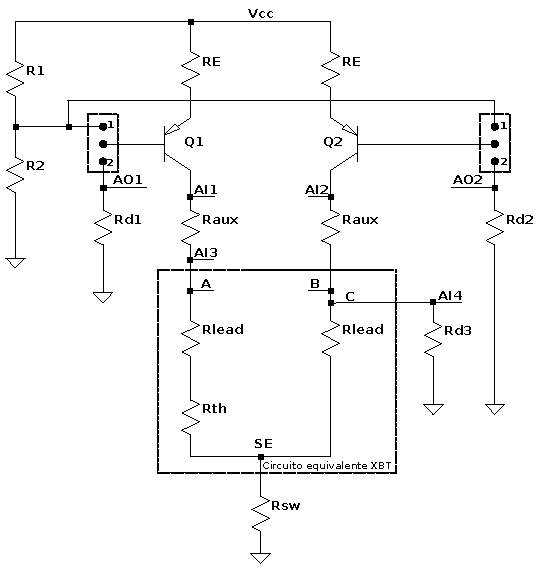
\includegraphics[width=.75\textwidth]{graficos/Disenio_definitivo_preliminar_2.pdf}
	\caption{Dise�o con dos fuentes de corriente, en el que se incluyen los dos esquemas de funcionamiento: la determinaci�n de $V_{BB}$ mediante un divisor resistivo y a trav�s de salidas anal�gicas del dispositivo adquisidor.}
	\label{fig_disenio_definitivo}
\end{figure}

En el esquema a lazo abierto, $V_{BB}$ queda determinada por un �nico divisor resistivo conectado a ambas bases de cada uno de los transistores que act�an como fuentes de corriente, tal como se observa en la FIG. \ref{fig_disenio_definitivo} (las bases de ambos transistores deben conectarse a la posici�n 1 de los selectores recuadrados). 

Se eligi� una combinaci�n de resistencias que, para una alimentaci�n de 5 V, lograran una tensi�n en el punto medio cercana al valor de dise�o y fueran, por un lado, lo suficientemente grandes como para evitar consumir una corriente innecesariamente grande y, por otro, lo suficientemente bajas como para no ser cargadas por la base de cada transistor cuando el XBT est� desconectado (modo \textit{reload}) o fuera del agua (modo \textit{launch}). 

En los modos \textit{reload} y \textit{launch}, el colector de cada transistor est� desconectado (el transistor no est� funcionando en MAD), pero la corriente de emisor se convierte en la corriente de base ya que el diodo emisor-base est� polarizado en directa. Esto provoca un aumento en la tensi�n en la base que puede atenuarse si la corriente de base es despreciable frente a la corriente del divisor resistivo. Si inicialmente se supone que la operaci�n del circuito auxiliar con el XBT en modos \textit{reload} o \textit{launch} no modifica la tensi�n en la base, la corriente de emisor, que coincide con la corriente de base, se mantendr� en 100 $\mu$A, lo que produce, considerando el efecto de ambos transistores, una inyecci�n de corriente en el divisor resistivo de 200 $\mu$A. Se escogieron resistencias de 680 $\Omega$ y 1 k$\Omega$, que consumen, en ausencia de efecto de carga por conexi�n de las bases de los transistores, una corriente de 3 mA, aproximadamente. De esta forma, el efecto de carga de la conexi�n de las bases de los transistores puede suponerse despreciable. La tensi�n $V_{BB}$, para los valores elegidos, queda establecida en aproximadamente 3 V. El valor exacto de $I_c$ se logra ajustando el \textit{preset} conectado al emisor. 

En el modo de funcionamiento a lazo cerrado (bases conectadas a la posici�n 2 de los selectores) las corrientes $I_c$ de ambas ramas son sensadas por dos pares de entradas anal�gicas, conectadas en ambos terminales de las resistencias $R_\text{aux}$ que se suponen conocidas y de precisi�n. Si el sistema adquisidor detecta un corrimiento respecto del valor de dise�o previsto para cualquiera de las corrientes actuar� modificando las tensiones en las bases de cada transistor, conectadas a salidas anal�gicas. De esta forma se garantiza, en tiempo de ejecuci�n, que las corrientes por ambas ramas sean iguales, lo que permite asegurar que la tensi�n $V_{AB}$ en la FIG. \ref{fig_principio_funcionamiento} se deba exclusivamente a la ca�da en $R_\text{th}$. 

Es importante destacar que para que las salidas anal�gicas puedan conectarse a las bases de transistores PNP, se debe utilizar resistencias de derivaci�n, conectadas a la base, para evitar corrientes entrantes (ver resistencias $R_\text{d1}$ y $R_\text{d2}$ en la FIG. \ref{fig_disenio_definitivo}).

Como fuera mencionado anteriormente, tanto en modo \textit{reload} o en modo \textit{launch} las ramas de ambos colectores est�n abiertas, es decir, sin un camino hacia tierra. Ambos transistores dejan de estar en MAD y la tensi�n $V_{EC}$ en cada uno de ellos vale cero. Al no haber corriente saliendo por los colectores, las ca�das de tensi�n en las resistencias $R_\text{aux}$ son nulas, lo que permite detectar que el sistema no est� midiendo. En este caso, las cuatro entradas anal�gicas perciben una tensi�n igual a $V_{CC} - V_{RE}$, que para las condiciones de dise�o est� entre 3,6 V y 3,8 V. Estos valores est�n dentro de los m�rgenes de seguridad de m�xima tensi�n admisible para entradas de microcontroladores que trabajan con 3,3 V. 

Para que el sistema logre diferenciar el modo \textit{launch} del modo \textit{reload}, se decidi� que la entrada anal�gica que sensa el terminal ubicado aguas abajo de la resistencia $R_\text{aux}$, en la rama que no contiene al termistor (indicada como AI4 en la FIG. \ref{fig_disenio_definitivo}), se conecte al nodo C del XBT. De esta forma, s�lo existe una conexi�n el�ctrica al terminal inferior de $R_\text{aux}$ cuando el XBT est� conectado (modo \textit{launch}). 

En modo \textit{reload} la entrada AI4 queda desconectada y, en caso de que se la vincule a tierra a trav�s de una resistencia de valor elevado ($R_\text{d3}$ en la FIG. \ref{fig_disenio_definitivo}), registar� un estado bajo (en torno a 0 V).

Los nodos de sensado se vincularon a las entradas anal�gicas a trav�s de amplificadores operacionales en modo seguidor por emisor. Se utiliz� el integrado LM324, que contiene cuatro \textit{op-amps} que funcionan con alimentaci�n simple (s�lo tensi�n positiva) y admiten tensiones de salida m�nimas muy cercanas a 0 V. Para los transistores se eligi� el modelo 2N3906, un transistor bipolar PNP de uso general para aplicaciones de baja potencia.

En la FIG. \ref{fig:esquematico_disenio_dos_fuentes} se muestra el circuito esquem�tico completo, dise�ado para integrarse al kit de desarrollo NUCLEO-STM32F429ZI. Este esquem�tico incluye una circuiter�a, armada con resistores, que emulan el comportamiento del termistor y permiten simular el funcionamiento del sistema en ausencia de una sonda XBT real, para en determinadas condiciones. 

El modo simulaci�n se logra cortocircuitando los pares de terminales 1-2, 3-4 y 5-6 del conector J3. Los resistores $R_7$ y $R_8$ representan las $R_\text{lead}$ de un XBT arbitrario. Los resistores $R_9$ y $R_{10}$ representan dos posibles valores dentro del rango de funcionamiento del termistor, asociados a dos valores de temperatura. Si se conectan en paralelo, se obtiene un valor adicional. El resistor $R_{11}$ y el \textit{preset} variable $R_\text{v3}$ se utilizan para estudiar el comportamiento en un rango amplio de variaci�n de la resistencia del termistor. La combinaci�n de ambos resistores proporciona un rango entre 4,7 k$\Omega$ y 14,7 k$\Omega$. 

El conector J7 permite simular el lanzamiento de una sonda XBT y su ingreso al agua de mar al cerrar un camino conductor a masa.

\begin{landscape}

	\begin{figure}[htpb]
	\centering 
	\vspace{-1cm}
	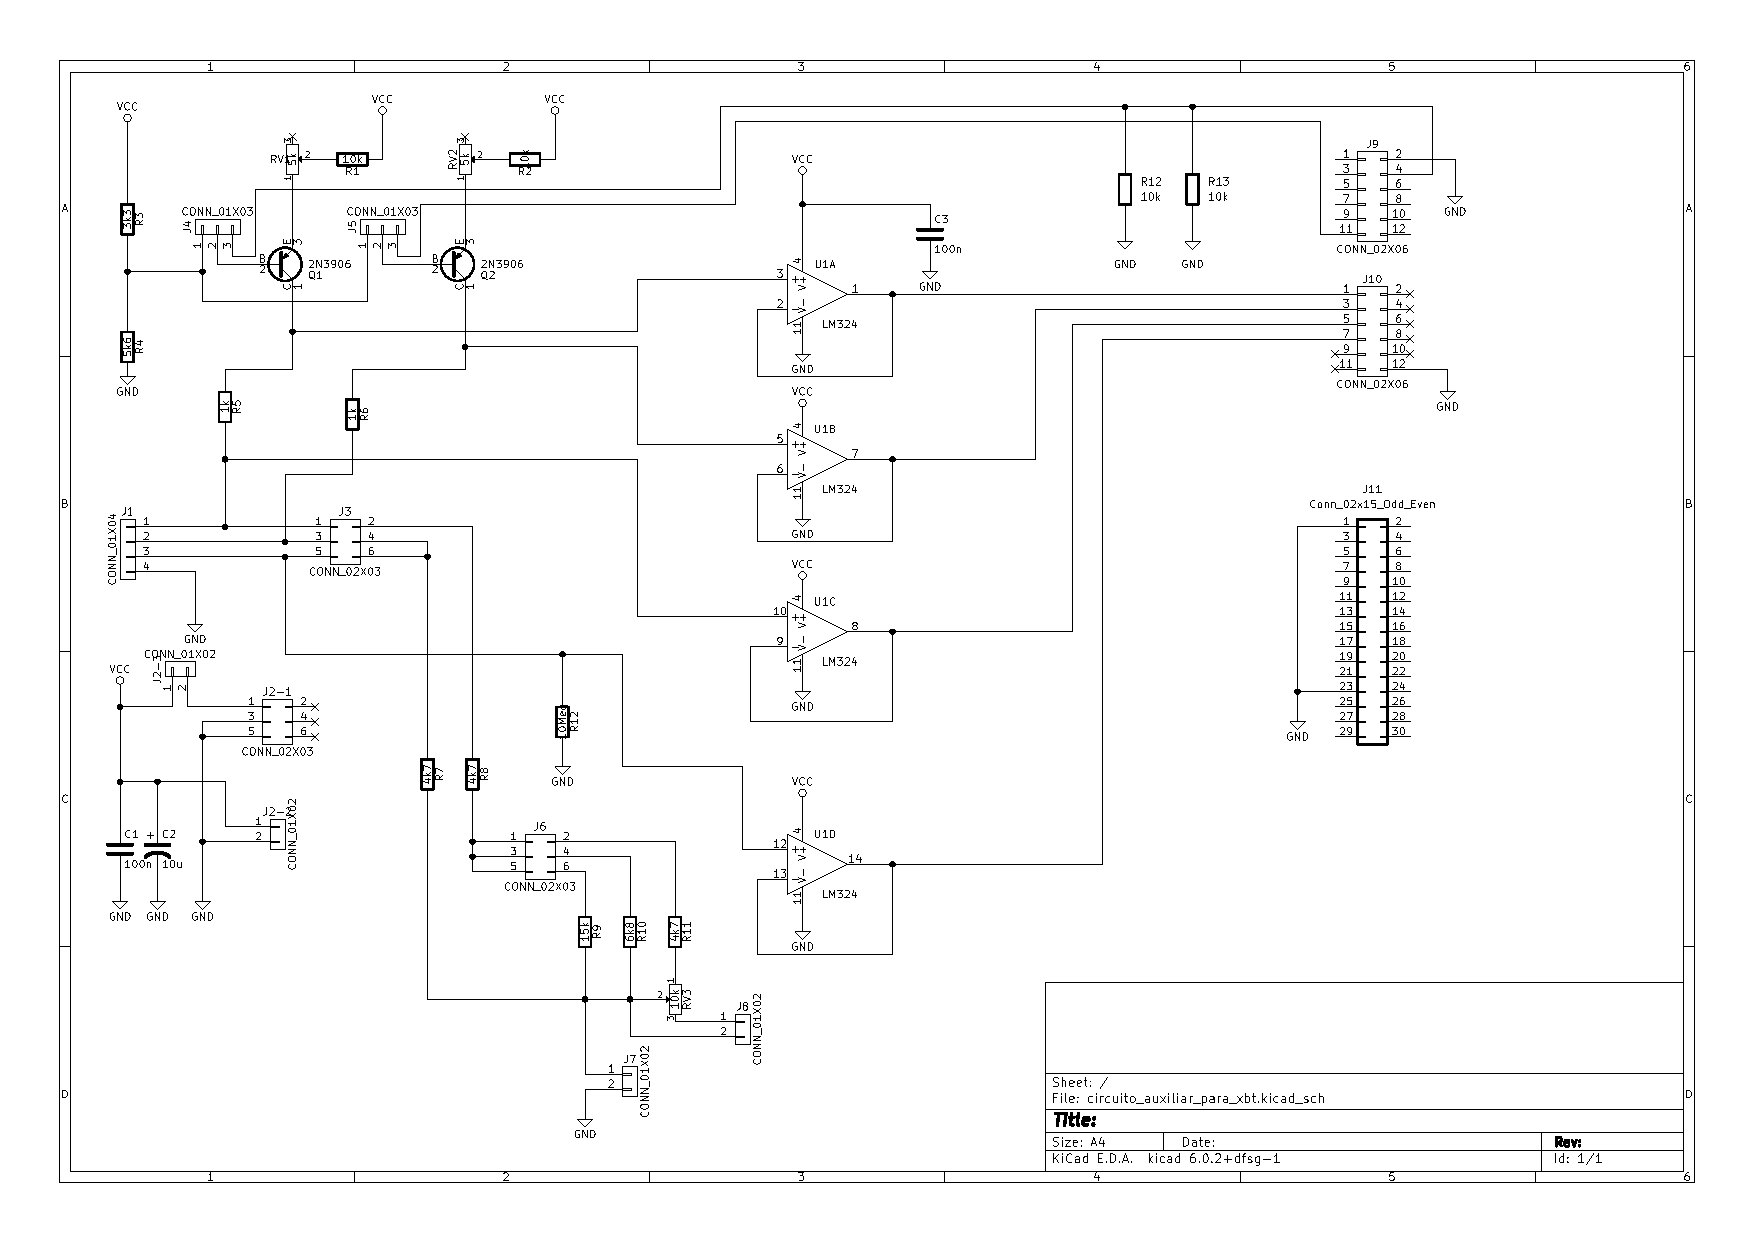
\includegraphics[height=1.\textheight]{./graficos/circuito_auxiliar_para_xbt.pdf}
	%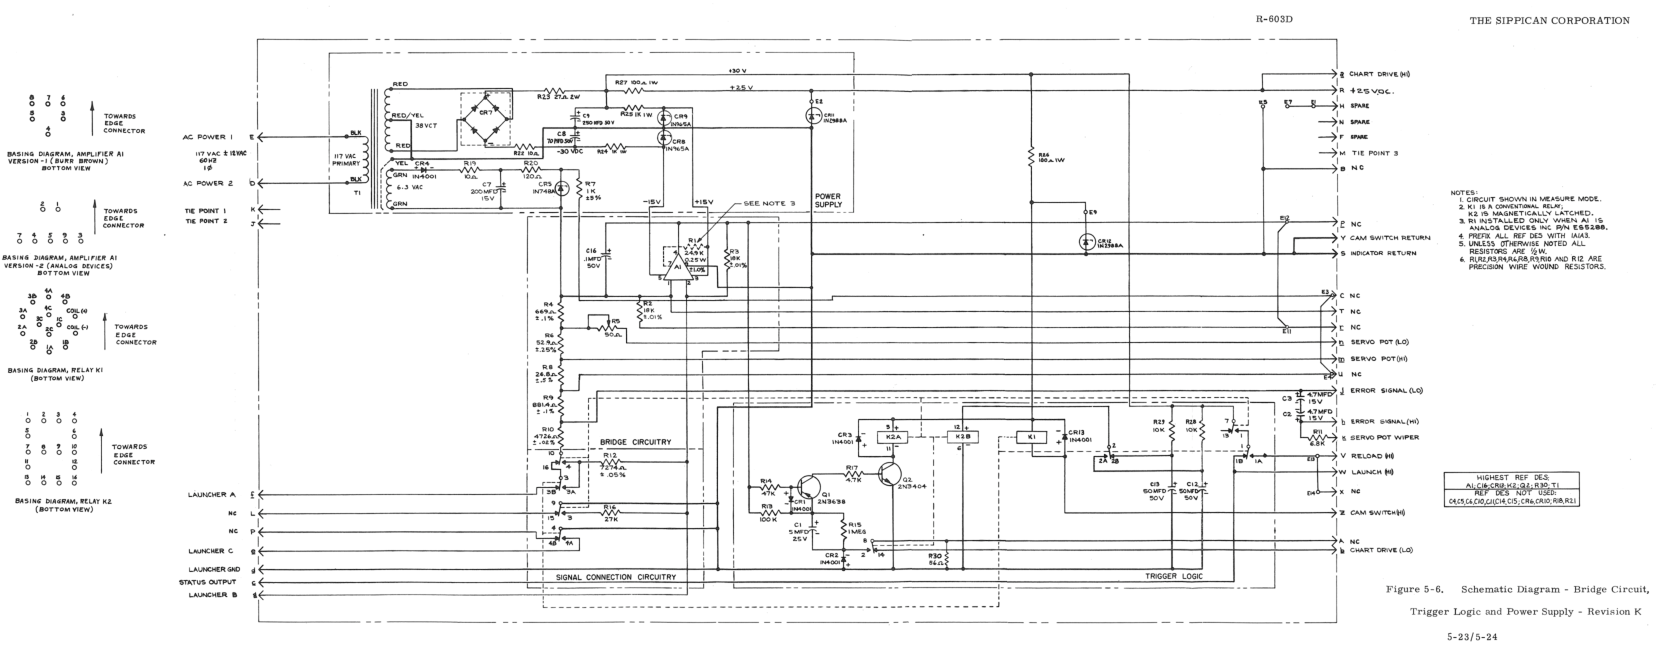
\includegraphics[width=1\textwidth]{./graficos/Esquematico_puente_recortado.pdf}
	\caption{Circuito esquem�tico completo del dise�o del circuito auxiliar con dos fuentes de corriente.}
	\label{fig:esquematico_disenio_dos_fuentes}
	\end{figure}

\end{landscape}

\subsubsection{Simulaciones del circuito de dos fuentes de corriente}

Se realizaron simulaciones del funcionamiento del circuito de dos fuentes de corriente. Los an�lisis llevados a cabo tienen como objetivo verificar el funcionamiento normal del dise�o y su robustez frente a modificaciones en algunos de los resistores que forman parte del dise�o.

La estimaci�n de la resistencia del termistor, $R_\text{th}$, que se desprende del circuito presentado en la FIG. \ref{fig_disenio_definitivo}, se obtiene mediante la expresi�n:

%\vspace{10px}
\begin{equation}
\tilde{R}_\text{th} = \frac{V_\text{ai3} - V_\text{ai4}}{V_\text{ai1} - V_\text{ai3}} R_\text{aux}
\label{ec:Rth_monio}
\end{equation}
%\vspace{10px}

\noindent donde $V_\text{ai3} - V_\text{ai4}$ coincide con la tensi�n $V_\text{AB}$, que a su vez es la ca�da en $R_\text{th}$ cuando las corrientes por ambas ramas son iguales y el cociente $(V_\text{ai1} - V_\text{ai3})/R_\text{aux}$ es la estimaci�n de la corriente por la rama que contiene al termistor. 

La calidad de la estimaci�n de la resistencia del termistor, $\tilde{R}_\text{th}$, depende fundamentalmente de la igualdad de las corrientes por ambas ramas y de que se garantice que ambos transistores est�n funcionando en MAD. Esto �ltimo puede dejar de cumplirse ante un aumento en las resistencias conectadas entre los colectores y el nodo com�n, con especial �nfasis en la rama que contiene el termistor. 

El valor de la corriente entregada por las fuentes de corriente se eligi� para garantizar que, a�n teniendo devanados cuya resistencia, $R_\text{lead}$ sea de 10 k$\Omega$, valor mayor que los que se encuentran en los XBT analizados, se evite caer en la regi�n de saturaci�n de los transistores. Esto se evidencia en la FIG. \ref{fig:sweep_Rlead}, que muestra un an�lisis del punto de operaci�n del sistema, considerando una $R_\text{th}$ variable entre los l�mites de variaci�n del termistor y un conjunto discreto de valores posibles de las $R_\text{lead}$, que se asumen apareadas en todo momento.

\vspace{30px}
\begin{figure}[htpb]
	\centering
	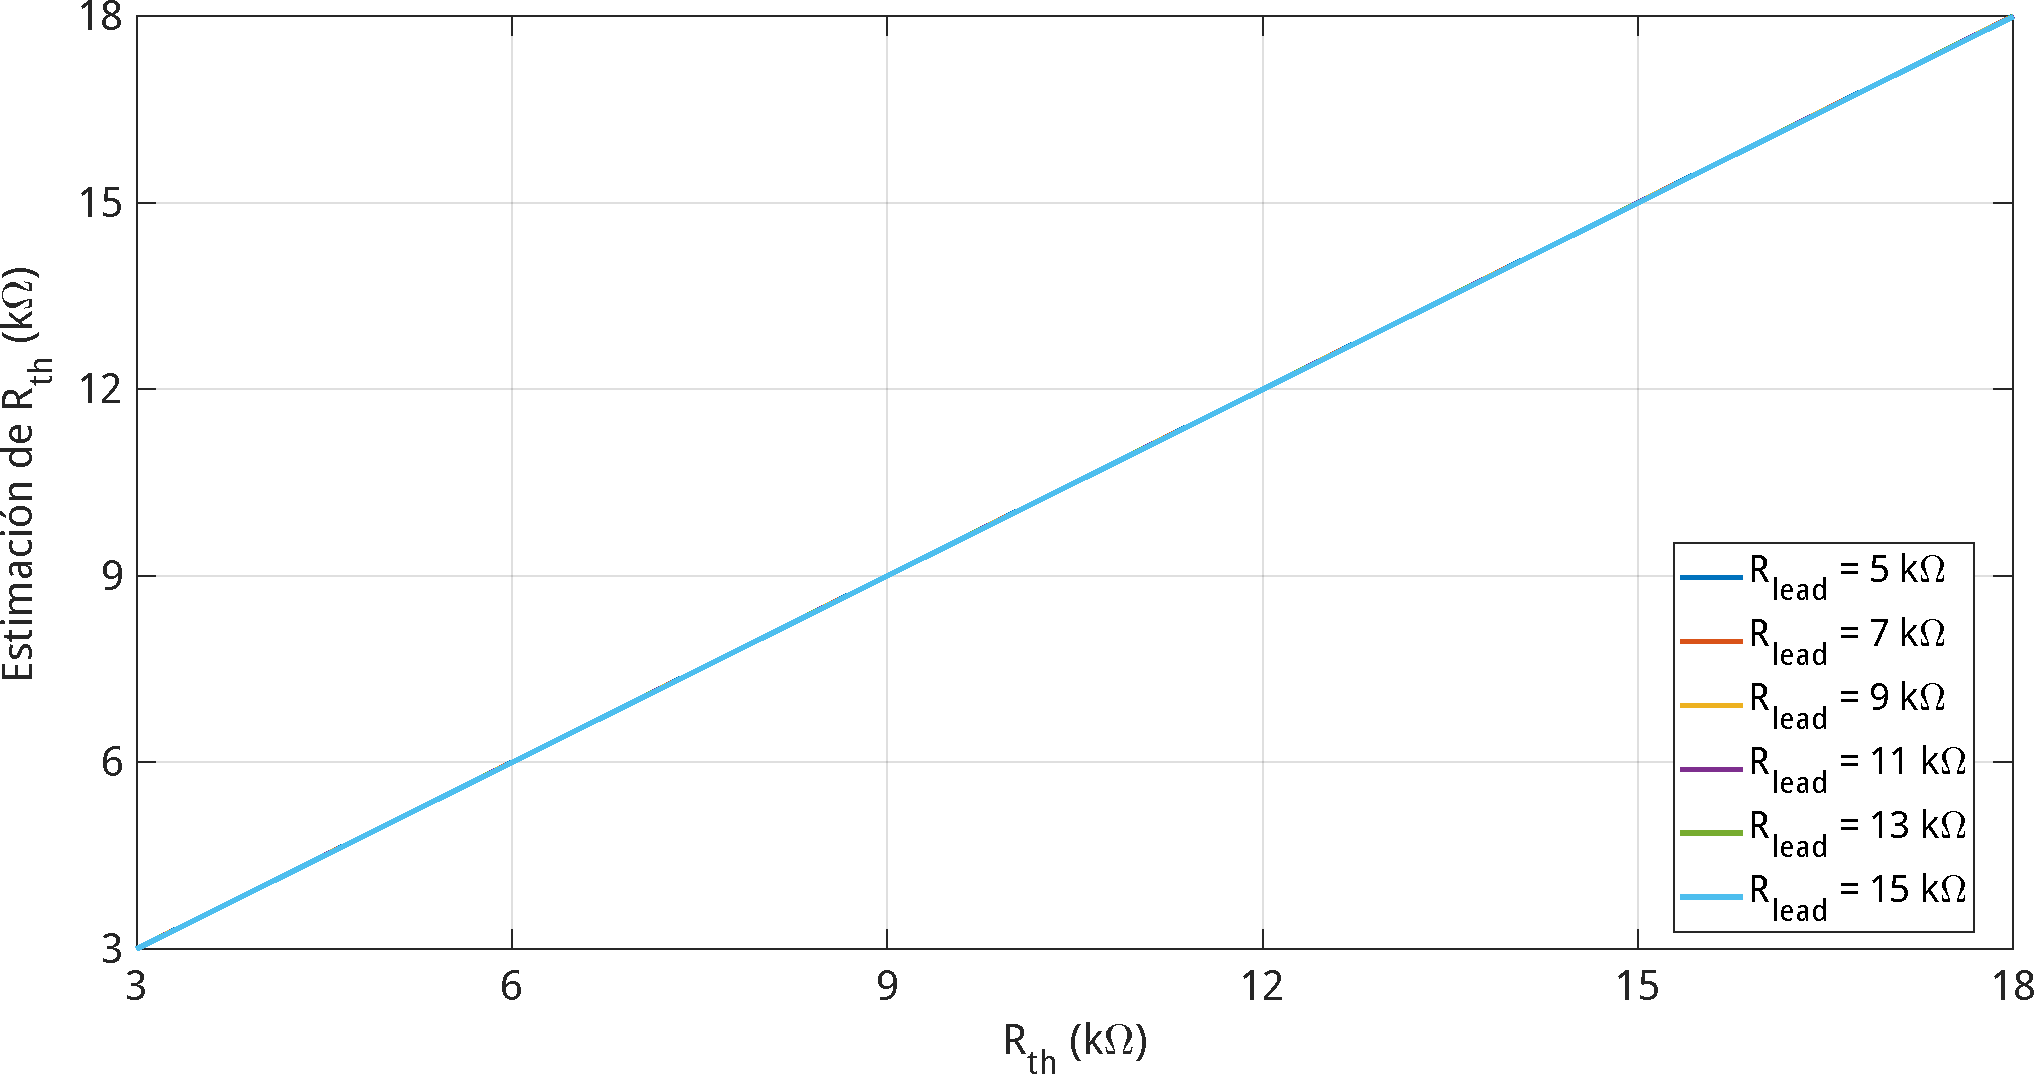
\includegraphics[width=\textwidth]{graficos/Variacion_Rlead.pdf}
	\caption{Estimaci�n de $R_\text{th}$ para distintos valores de $R_\text{lead}$.}
	\label{fig:sweep_Rlead}
\end{figure}
\vspace{30px}

La simulaci�n mostrada se realiz� considerando una resistencia equivalente del agua de mar, $R_\text{sw}$ de 1 $\Omega$, valor despreciable con respecto a las resistencias de cada una de las ramas. Como puede observarse, a�n para $R_\text{lead} =$ 15 k$\Omega$, el cual resulta casi exagerado, es posible recuperar el valor de $R_\text{th}$ pr�cticamente en su valor real (en ausencia de otras fuentes de incerteza). 

El an�lisis se repiti� para $R_\text{lead}$ fija en 10 k$\Omega$ y una variaci�n de $R_\text{sw}$ entre 1 $\Omega$ y 1 k$\Omega$. Este �ltimo valor se utiliz� como margen de seguridad, ya que se supone mucho mayor que la resistencia efectiva del agua de mar entre el electrodo de contacto del XBT y el casco de la embarcaci�n. Los resultados se muestran en la FIG. \ref{fig:sweep_Rsw}.

\vspace{30px}
\begin{figure}[htpb]
	\centering
	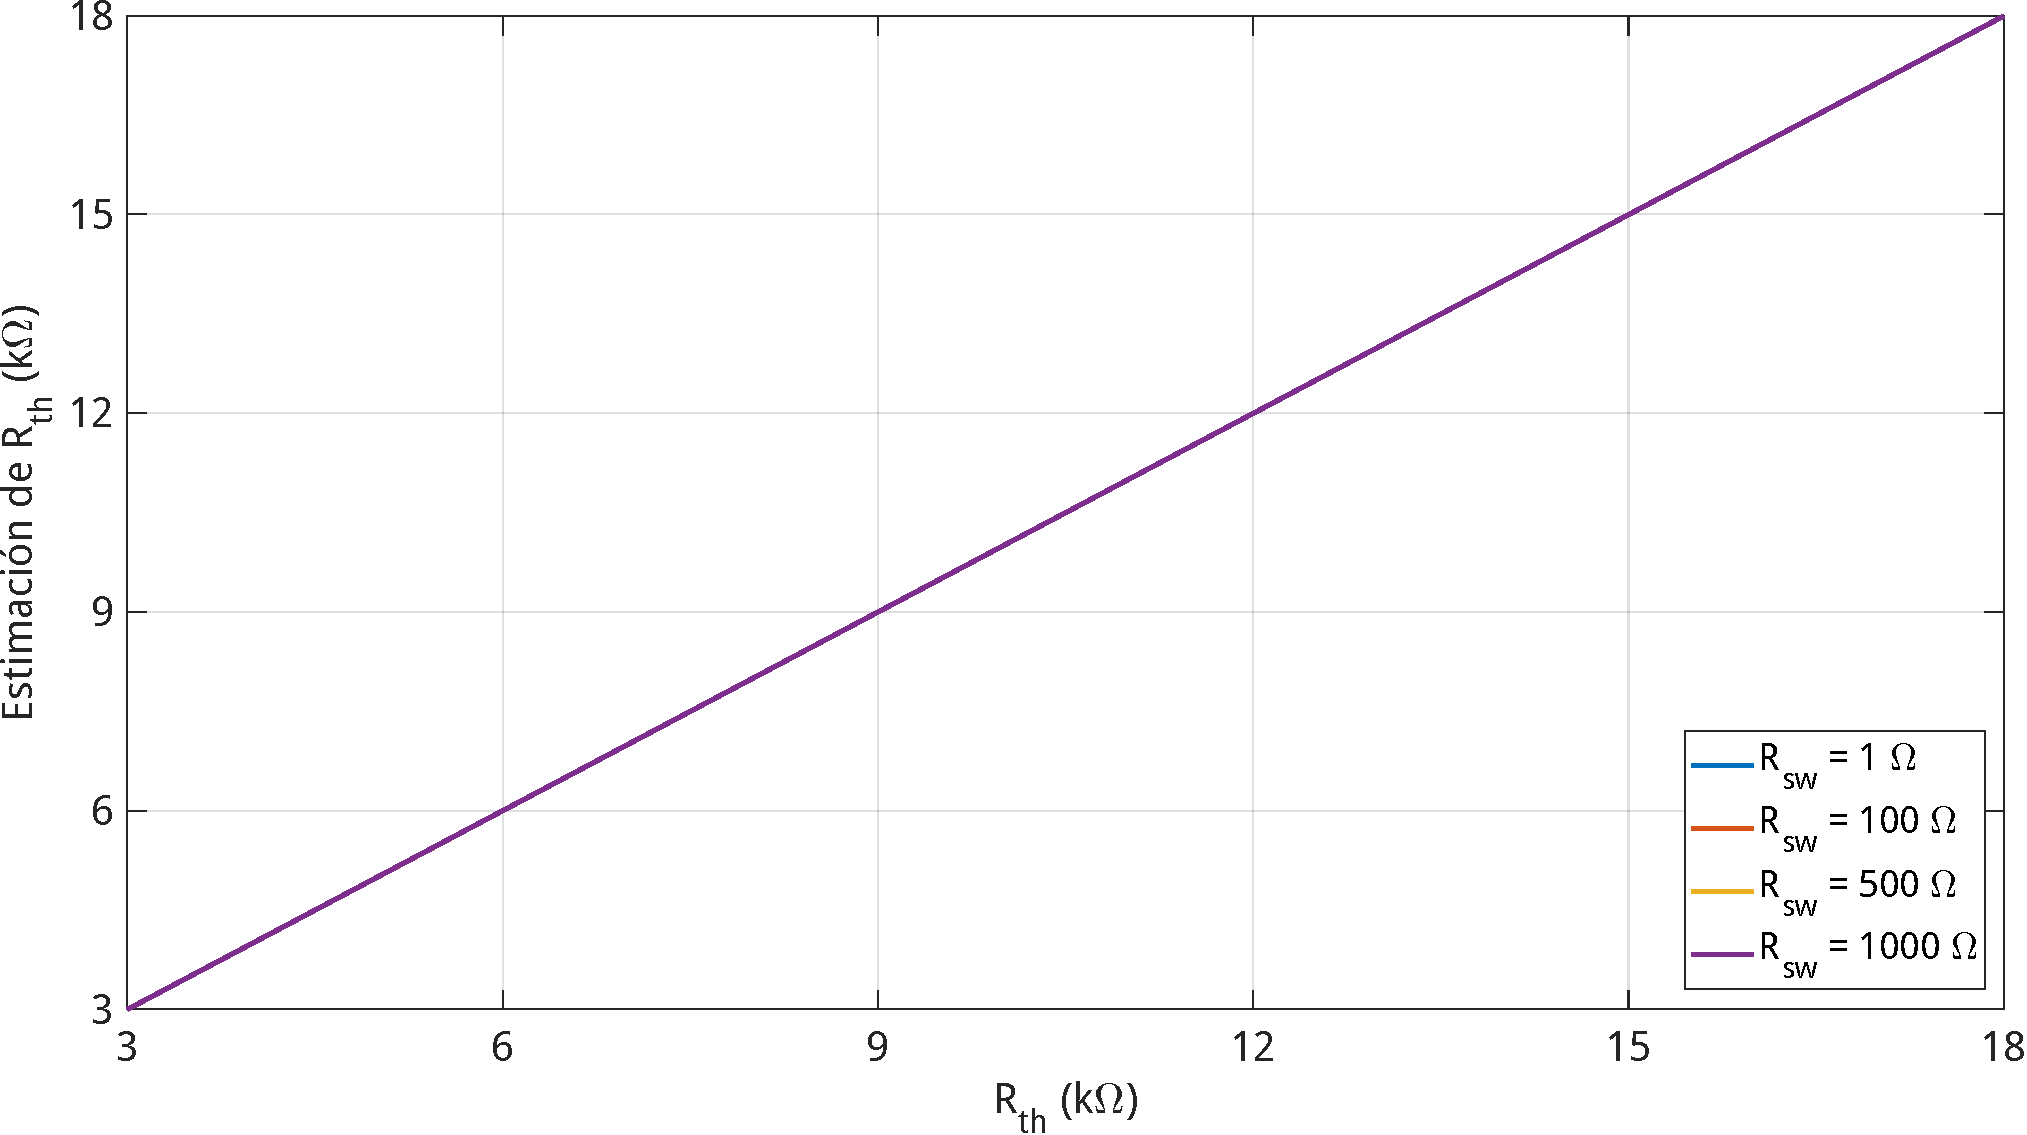
\includegraphics[width=\textwidth]{graficos/Variacion_Rsw.pdf}
	\caption{Estimaci�n de $R_\text{th}$ para distintos valores de $R_\text{sw}$.}
	\label{fig:sweep_Rsw}
\end{figure}
\vspace{30px}

Del mismo modo que para la variaci�n de $R_\text{lead}$, se observa que la estimaci�n de $R_\text{th}$ no se ve afectada para los distintos valores propuestos de $R_\text{sw}$. 

Se realizaron, adicionalmente, an�lisis de sensibilidad teniendo en cuenta variaciones del conjunto de resistencias que conforman la malla de entrada de los transistores y que est�n intr�nsecamente relacionadas con la determinaci�n de las corrientes de ambas fuentes. 

Inicialmente se simul� una variaci�n las resistencia $R_2$ del divisor resistivo que determina la tensi�n en la bases de los transistores, con un margen de incerteza del 10\% respecto del valor nominal. Se consider� un valor para $R_1$, que permaneci� fija, de 748 $\Omega$ (10\% mayor que su valor nominal, de 680 $\Omega$), ya que el efecto combinado de aumento de $R_1$ y la disminuci�n de $R_2$ provoca un aumento de la corriente de las fuentes, lo que reduce el rango de posibles cargas que pueden conectarse en el colector de la rama que contiene al termistor. Los resultados se muestran en la FIG. \ref{fig:sweep_R2}

\vspace{30px}
\begin{figure}[!hbt]
	\centering
	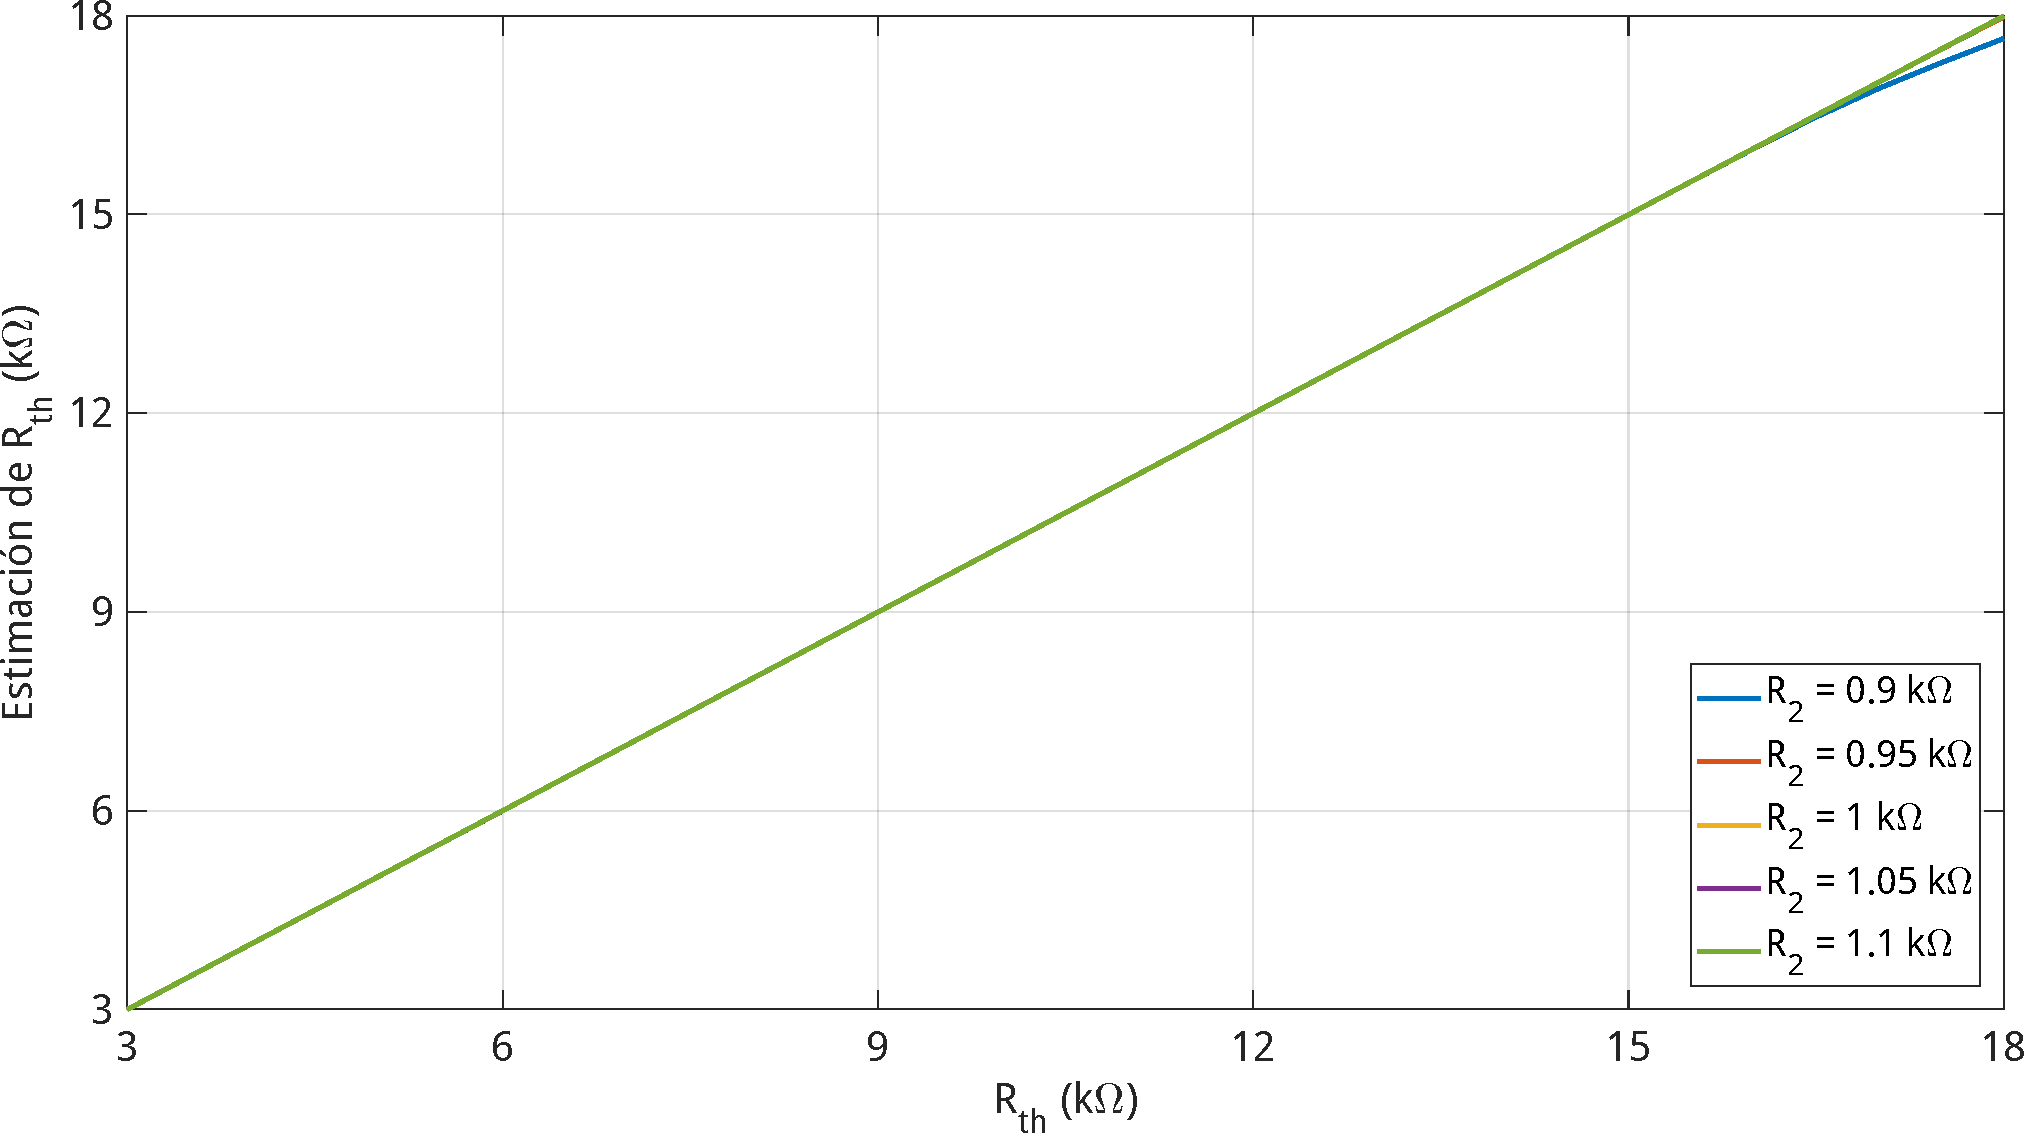
\includegraphics[width=\textwidth]{graficos/Variacion_R2_con_R1_al_90porciento.pdf}
	\caption{Estimaci�n de $R_\text{th}$ para distintos valores de $R_2$, considerando un incremento para $R_1$ del 10\% respecto de su valor nominal.}
	\label{fig:sweep_R2}
\end{figure}
\vspace{30px}

Se observa que para pr�cticamente todos los posibles valores de $R_2$, dentro del margen de incerteza propuesto, es posible recuperar $R_\text{th}$ con exactitud. Queda execptuado el caso de $R_2$ = 900 $\Omega$, donde se empieza a observar un corrimiento en la estimaci�n para los valores mayores de $R_\text{th}$, como consecuencia de que la corriente, en la rama que contiene al termistor, no puede aumentar proporcionalmente a la ca�da en $R_E$, debido a que el transistor $Q_1$ deja de estar en MAD. Para el caso l�mite de $R_\text{th}$ = 18 k$\Omega$, la estimaci�n obtenida arroja un valor de 17,65 k$\Omega$, el cual representa un error del 2\%, aproximadamente. Esto deja en evidencia la ventaja de utilizar el esquema de funcionamiento a lazo cerrado.

Uno de los an�lisis m�s importantes para estudiar la robustez del prototipo implica la variaci�n de las resistencias de emisor, $R_E$. La variaci�n de una de ellas respecto de la otra (se las denominar�, de ahora en adelante, $R_{E1}$ y $R_{E2}$) provoca que las corrientes de ambas fuentes no sean iguales, lo que degrada la estimaci�n de $R_\text{th}$. En la FIG. \ref{fig:sweep_RE1} se muestra dicha estimaci�n, en funci�n del valor real de $R_\text{th}$, para varios valores posibles de $R_{E1}$ y considerando un valor de $R_{E2}$ igual al valor nominal de dise�o.

\begin{figure}[htpb]
	\centering
	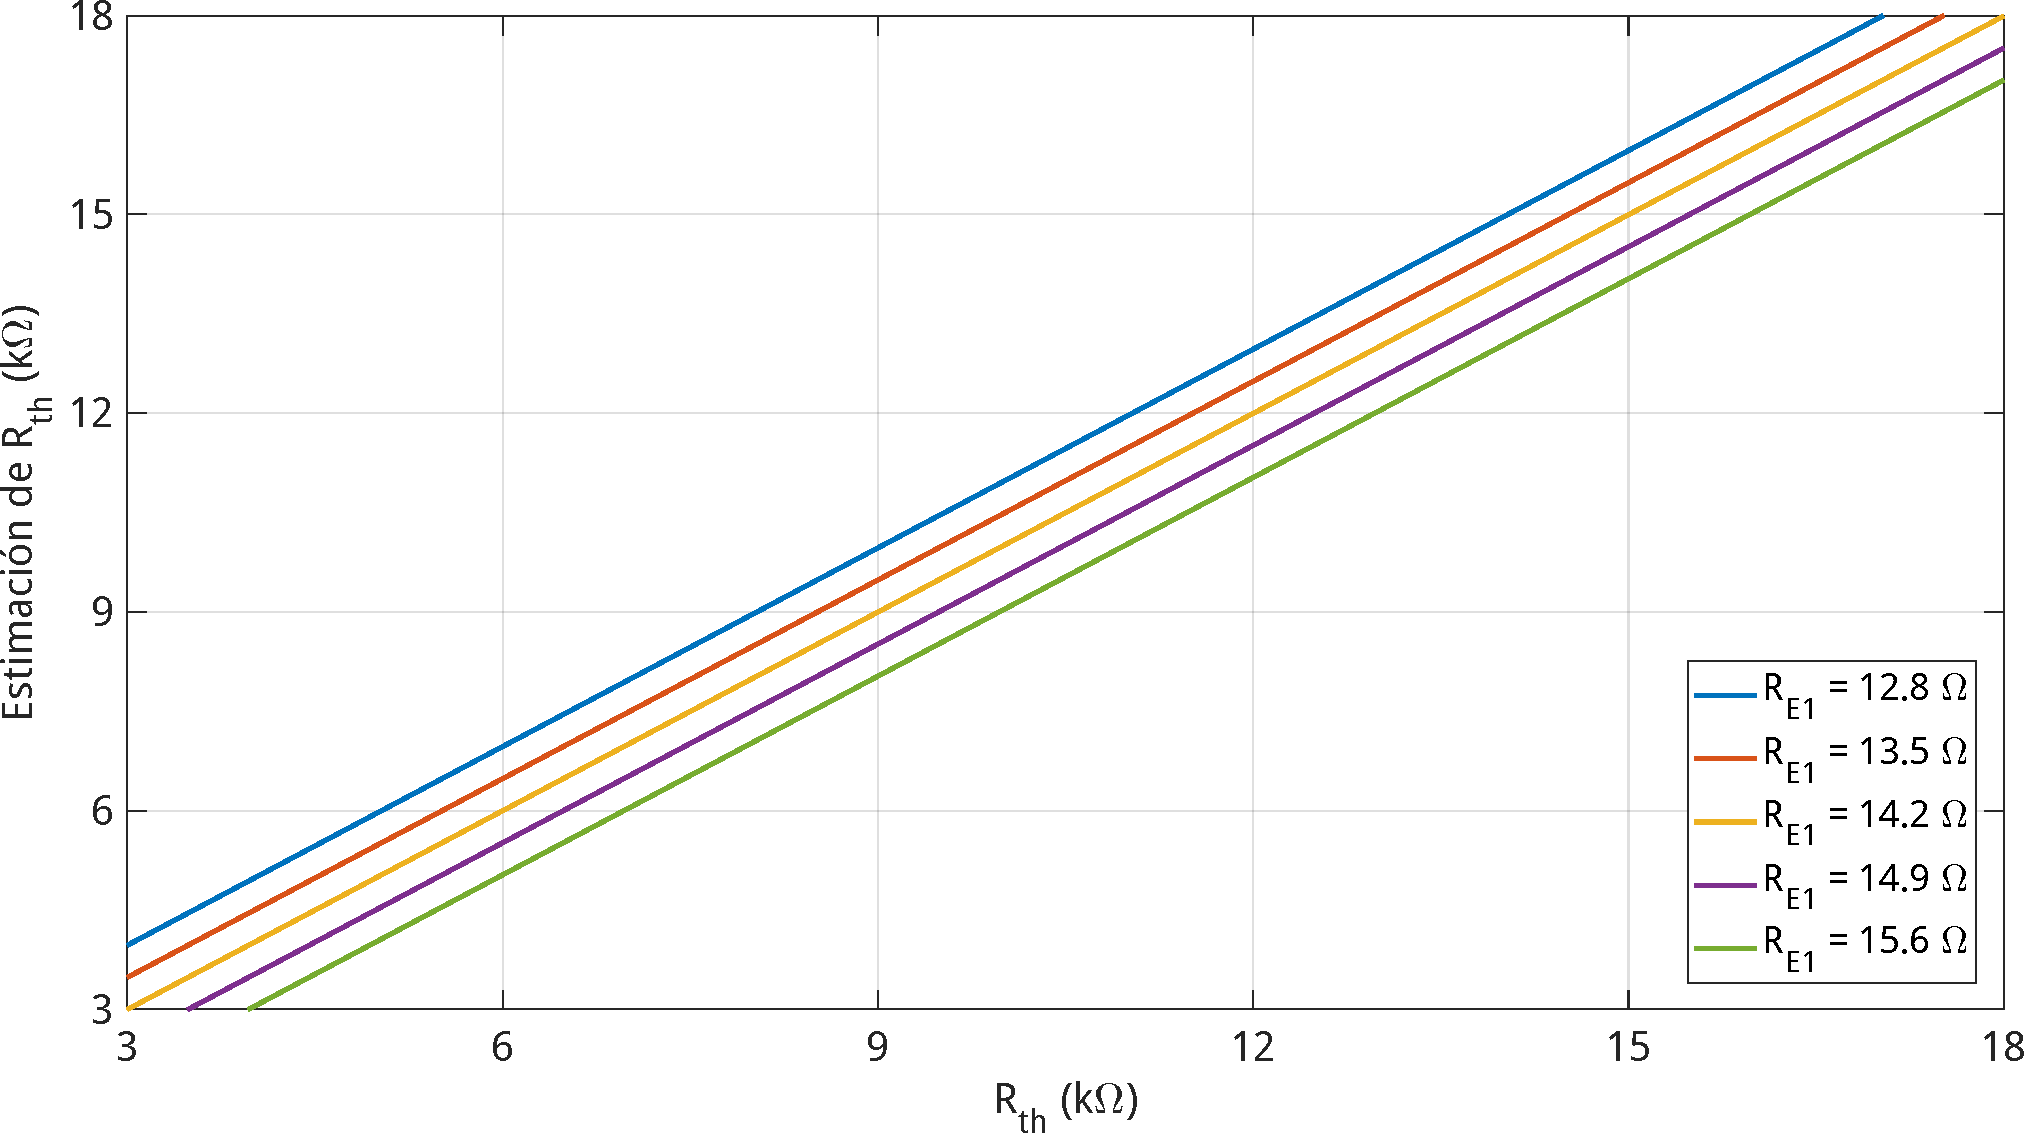
\includegraphics[width=\textwidth]{graficos/Variacion_RE1.pdf}
	\caption{Estimaci�n de $R_\text{th}$ para distintos valores de $R_E1$, en torno al 10\% de su valor nominal.}
	\label{fig:sweep_RE1}
\end{figure}

Se observa una variabilidad significativa en todo el rango de posibles valores de resistencia del termistor. Como el \textit{mismacth} de corrientes de ambas fuentes genera un corrimiento fijo en la estimaci�n respecto del valor verdadero, su error relativo se incrementa para las resistencias de termistor m�s bajas (asociadas a temperaturas m�s altas). 

Cuando se desea estimar un valor de $R_\text{th}$ del orden de los 3 k$\Omega$ ante un corrimiento del 10\% en el valor nominal de $R_{E1}$, el error relativo asciende al 32\%. Esto deja en evidencia la necesidad de abordar el esquema de funcionamiento a lazo cerrado, o a utilizar resistores de precisi�n, en vez de series de resistores y \textit{presets}, para las resistencias de emisor. Un resultado similar se obtiene cuando se analiza el desempe�o del circuito ante variaciones de $R_{E2}$, manteniendo $R_{E1}$ fija. Esto se muestra en la FIG. \ref{fig:sweep_RE2}.


\begin{figure}[htpb]
	\centering
	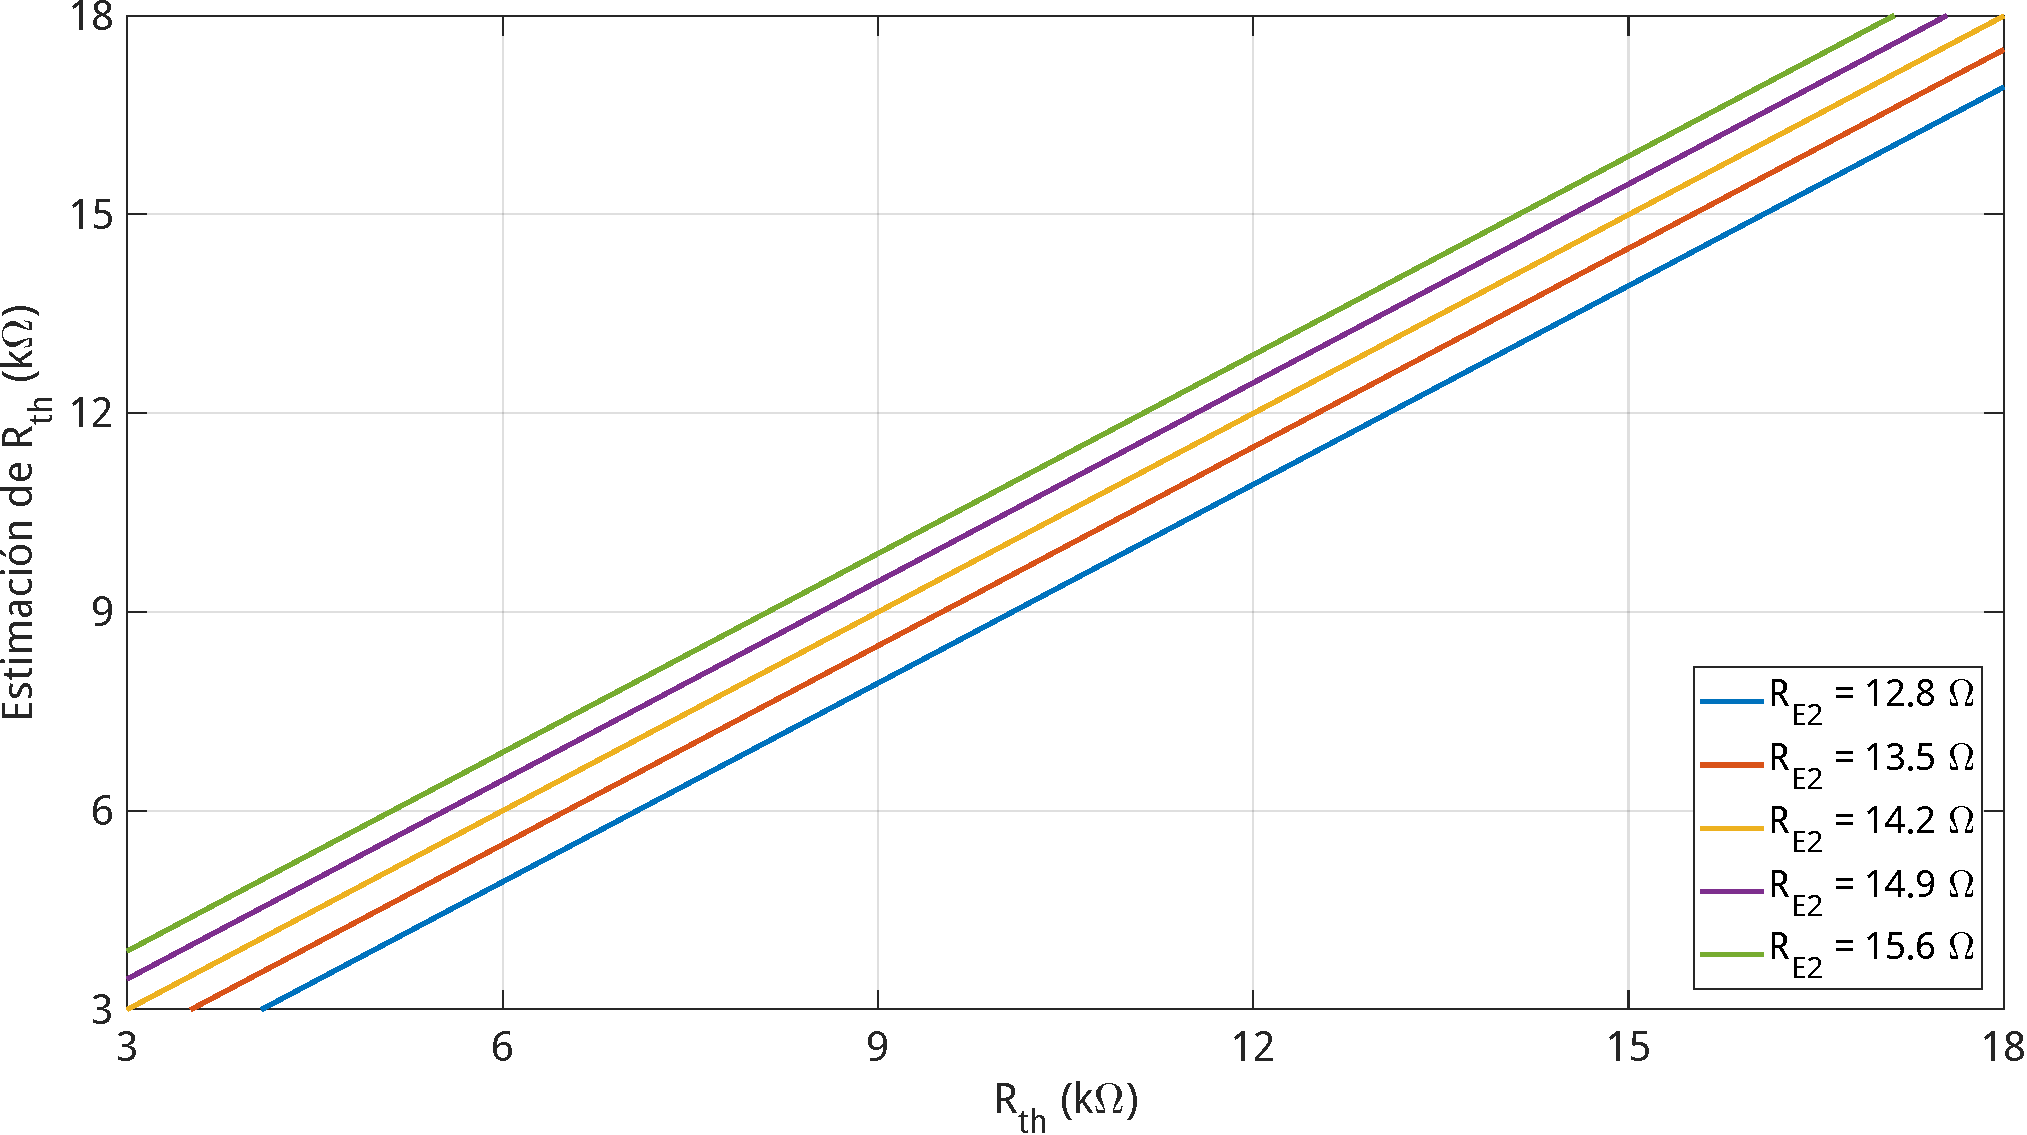
\includegraphics[width=\textwidth]{graficos/Variacion_RE2.pdf}
	\caption{Estimaci�n de $R_\text{th}$ para distintos valores de $R_E2$, en torno al 10\% de su valor nominal.}
	\label{fig:sweep_RE2}
\end{figure}





\clearpage
\subsection{Puente balanceado JFET}

Se analiz� la conveniencia de utilizar una topolog�a circuital descripta en la literatura \citep{STEGEN1975447} que forma parte de un sistema port�til de digitalizaci�n y registro XBT, desarrollado en la d�cada del setenta. Si bien ha habido grandes avances tecnol�gicos, especialmente en el campo de la electr�nica desde ese tiempo a la fecha, el principio de funcionamiento sigue siendo v�lido y aplicable en la actualidad si se reemplazan los componentes originales por componentes modernos, funcionalmente equivalentes.

El circuito analizado es un puente auto-balanceado que utiliza un transistor de efecto de campo, JFET, realimentado, para ``copiar'' permanentemente el valor de la resistencia del termistor en la sonda XBT y producir una tensi�n de salida linealmente proporcional a esta en todo su rango de operaci�n. 

En la FIG. \ref{fig:stegen}, se muestra un circuito esquem�tico simplificado en el que se puede apreciar el puente auto-balanceado conectado al circuito equivalente el�ctrico de la sonda XBT, representado por el resistor del termistor y dos resistores para las resistencias de los devanados que el fabricante garantiza que se encuentran precisamente apareados en un valor pr�ximo a 5 k$\Omega$.  

\begin{figure}[htpb]
	\centering
	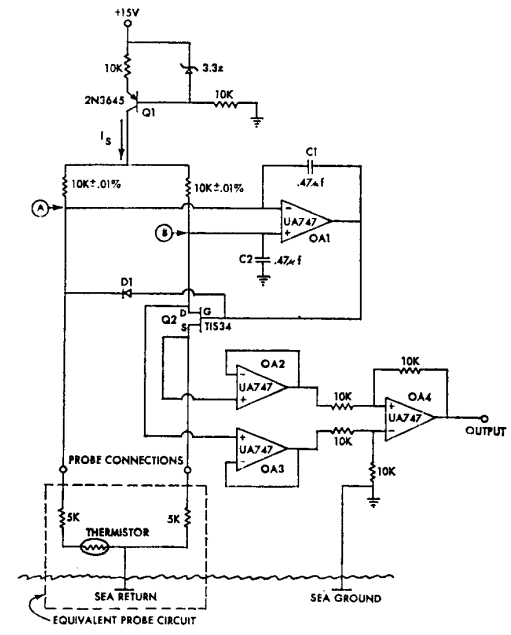
\includegraphics[width=0.75\textwidth]{graficos/self_balancing_bridge.png}
	\caption{Diagrama esquem�tico del circuito puente auto-balanceado.}
	\label{fig:stegen}
\end{figure}  

El circuito del puente esta formado por diferentes sub-bloques, a saber: una fuente de corriente constante , un amplificador operacional que controla el \textit{gate} del transistor JFET Q2 y un conjunto de amplificadores operacionales para extraer una tensi�n proporcional al valor de resistencia del termistor sin afectar el balance ni el normal funcionamiento del puente.

La fuente de corriente constante se implementa con el transistor Q1, polarizado para suministrar $I_S = 250\; \mu A$. Esta corriente se reparte en partes iguales por las dos ramas del puente debido a que la suma de las impedancias de cada rama est� precisamente apareada por dise�o. Para que esto se cumpla, los resistores de 10 K$\Omega$ en la parte superior del puente deben ser elementos de precisi�n, con baja dispersi�n en su resistencia respecto al valor nominal.

El amplificador operacional OA1 sensa la diferencia de potencial entre los puntos indicados como A y B del circuito y fuerza la resistencia del transistor Q2 a igualar la resistencia del termistor y as� el puente permanece balanceado.  Debido a que la corriente por Q2 es constante e igual a $0,5 \cdot I_S$, su resistencia se puede obtener midiendo la tensi�n entre \textit{drain} y \textit{source}, $V_{DS}$. 

El amplificador operacional OA4 funciona en configuraci�n amplificador diferencial con los amplificadores operacionales OA2 y OA3 en configuraci�n de \textit{buffers} de entrada y el conjunto produce una salida de tensi�n proporcional a la resistencia del transistor Q2 sin afectar el equilibrio del puente. Esta configuraci�n tambi�n se utiliza en el circuito descripto en la secci�n \ref{subsubsec:ampDiferencial} y se puede ver en la FIG. \ref{fig:opAmp_diferencial_2}.  

La salida del circuito se indica como OUTPUT y puede demostrarse que cuando los cuatro resistores en torno a OA4 tienen el mismo valor, es igual a:

\begin{equation}
OUTPUT = V_D - V_S,
\end{equation} 

\noindent la diferencia de potencial entre \textit{drain} y \textit{source} del transistor JFET, Q2, que a su vez es igual a la ca�da de potencial en el resistor del elemento sensor de la sonda XBT, $V_{THERMISTOR}$.

En la FIG. \ref{fig:puenteJFET} se presenta el circuito esquem�tico completo del puente.  Se puede apreciar que los amplificadores operacionales del puente utilizan alimentaci�n $\pm15 V.$, lo cual le agrega mayor complejidad al dise�o que requerir� una fuente de alimentaci�n partida frente a los dise�os que utilizan fuente simple con un �nico valor positivo.

El transistor Q1 que se utiliza en la fuente de corriente, es un transistor bipolar de juntura tipo PNP de peque�a se�al para prop�sitos generales.  Se utiliza para las simulaciones el modelo original 2N3645 que se puede reemplazar por un componente activo equivalente como el transistor 2N2907A \citep{2N2907A}, entre otros.

\vspace{2cm}
NOTAS PARA CONTINUAR:

Asimismo, en en circuito JFET 2N3823 en reemplazo del TIS34

UA741 opAmp cu�druple

Estimaci�n de Rth como Vout/(1/2*Is) = Vout/127,65 uA


\begin{figure}[htpb]
	\centering
	\includegraphics[width=0.9\textwidth]{graficos/puenteJfet.png}
	\caption{Circuito esquem�tico completo del puente auto-balanceado con valores de componentes actuales.}
	\label{fig:puenteJFET}
\end{figure}  

%Este dise�o tiene la ventaja de producir una tensi�n linealmente proporcional al valor de resistencia del termistor para todo el rango de temperatura.




\clearpage
\section{ENSAYOS}
\label{sec:simulaci�n}

Se fabric� un lote de circuitos impresos de doble capa en material FR4 con el dise�o del circuito con dos fuentes de corriente para evaluar su \textit{performance}.  El dise�o del PCB y el routeo de componentes se realiz� siguiendo recomendaciones generales para circuitos anal�gicos \citep{khandpur2006printed}. En la FIG. \ref{fig:PCB_montado} se observa un ejemplar de las placas fabricadas, con los componentes montados, integrada en el kit de desarrollo.

AGREGAR CONSIDERACIONES DE DISE�O PARA EL PCB:\\
 * MODO DE CONEXI�N CON LA NUCLEO A TRAV�S DE LOS HEADERS\\
 * MODO DE ALIMENTACI�N\\
 * JUMPERS Y SELECTORES\\
 * ENTRADA DE SE�ALES DE LA SONDA\\
 

\begin{figure}[htpb]
	\centering
	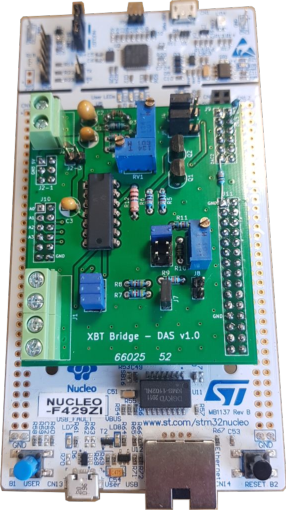
\includegraphics[width=0.35\textwidth]{graficos/PCB_mounted.pdf}
	\caption{Circuito impreso fabricado y montado en el kit de desarrollo utilizado como interfaz para el XBT.}
	\label{fig:PCB_montado}
\end{figure}

\subsection{Ensayos de laboratorio}

Se realiz� un conjunto de ensayos sobre la soluci�n circuital que emplea dos fuentes de corriente. Se us� el propio simulador de XBT incorporado en el circuito. Algunos resistores se midieron previamente a ser soldados al circuito impreso con un mult�metro GW Instek GDM-396, disponible en el DPA, a efectos de obtener una mejor estimaci�n de su resistencia. 

Se listan a continuaci�n los valores medidos, y el resto de los resistores utilizados (se asume, en los casos restantes, que es v�lido el valor nominal). En todos los casos se usaron resistores de metalfilm al 1\%. Sus identificadores se corresponden con el esquem�tico de la FIG. \ref{fig:esquematico_disenio_dos_fuentes}.

\begin{table}[htpb]
\centering
\caption{Resistores utilizados en el prototipo a ensayar.}
\label{tabla:ensayo}
\begin{tabular}{c|c|c|c}
Idetificador & Funci�n & Valor nominal & Valor medido \\ \hline
$R_1$ & $R_E$ fija lado A & 10 k$\Omega$ & - \\
$R_2$ & $R_E$ fija lado B & 10 k$\Omega$ & - \\
$R_\text{V1}$ & $R_E$ variable lado A & preset 5 k$\Omega$ & - \\
$R_\text{V2}$ & $R_E$ variable lado B & preset 5 k$\Omega$ & - \\
$R_3$ & $R_1$ del divisor & 560 $\Omega$ & 556 $\Omega$ \\
$R_3$ & $R_2$ del divisor & 820 $\Omega$ & 817 $\Omega$ \\
$R_5$ & $R_\text{aux}$ lado A & 1 k$\Omega$ & 992 $\Omega$ \\
$R_6$ & $R_\text{aux}$ lado B & 1 k$\Omega$ & 992 $\Omega$ \\
$R_7$ & $R_\text{lead}$ lado A & 5,6 k$\Omega$ & 5,57 k$\Omega$ \\
$R_8$ & $R_\text{lead}$ lado B & 5,6 k$\Omega$ & 5,57 k$\Omega$ \\
$R_9$ & $R_\text{th}$ Temp. fija 1 & 15 k$\Omega$ & 14,88 k$\Omega$ \\
$R_10$ & $R_\text{th}$ Temp. fija 2 & 6,8 k$\Omega$ & 14,88 k$\Omega$ \\

\end{tabular}
\end{table}

Adicionalmente, se emple� un resistor de 12 M$\Omega$ para el canal que mide el nodo C y dos resistores de valor nominal 10 k$\Omega$ como resistores de derivaci�n.

Se arm� un banco experimental formado por una fuente de laboratorio, mediante la que se aliment� el prototipo con 5 V, y un mult�metro para medir las tensiones que registrar�an las entradas anal�gicas del circuito digitalizador (no implementado en este ensayo). El banco se muestra en la FIG. \ref{fig:banco_exp}.

 \begin{figure}[htpb]
	\centering
	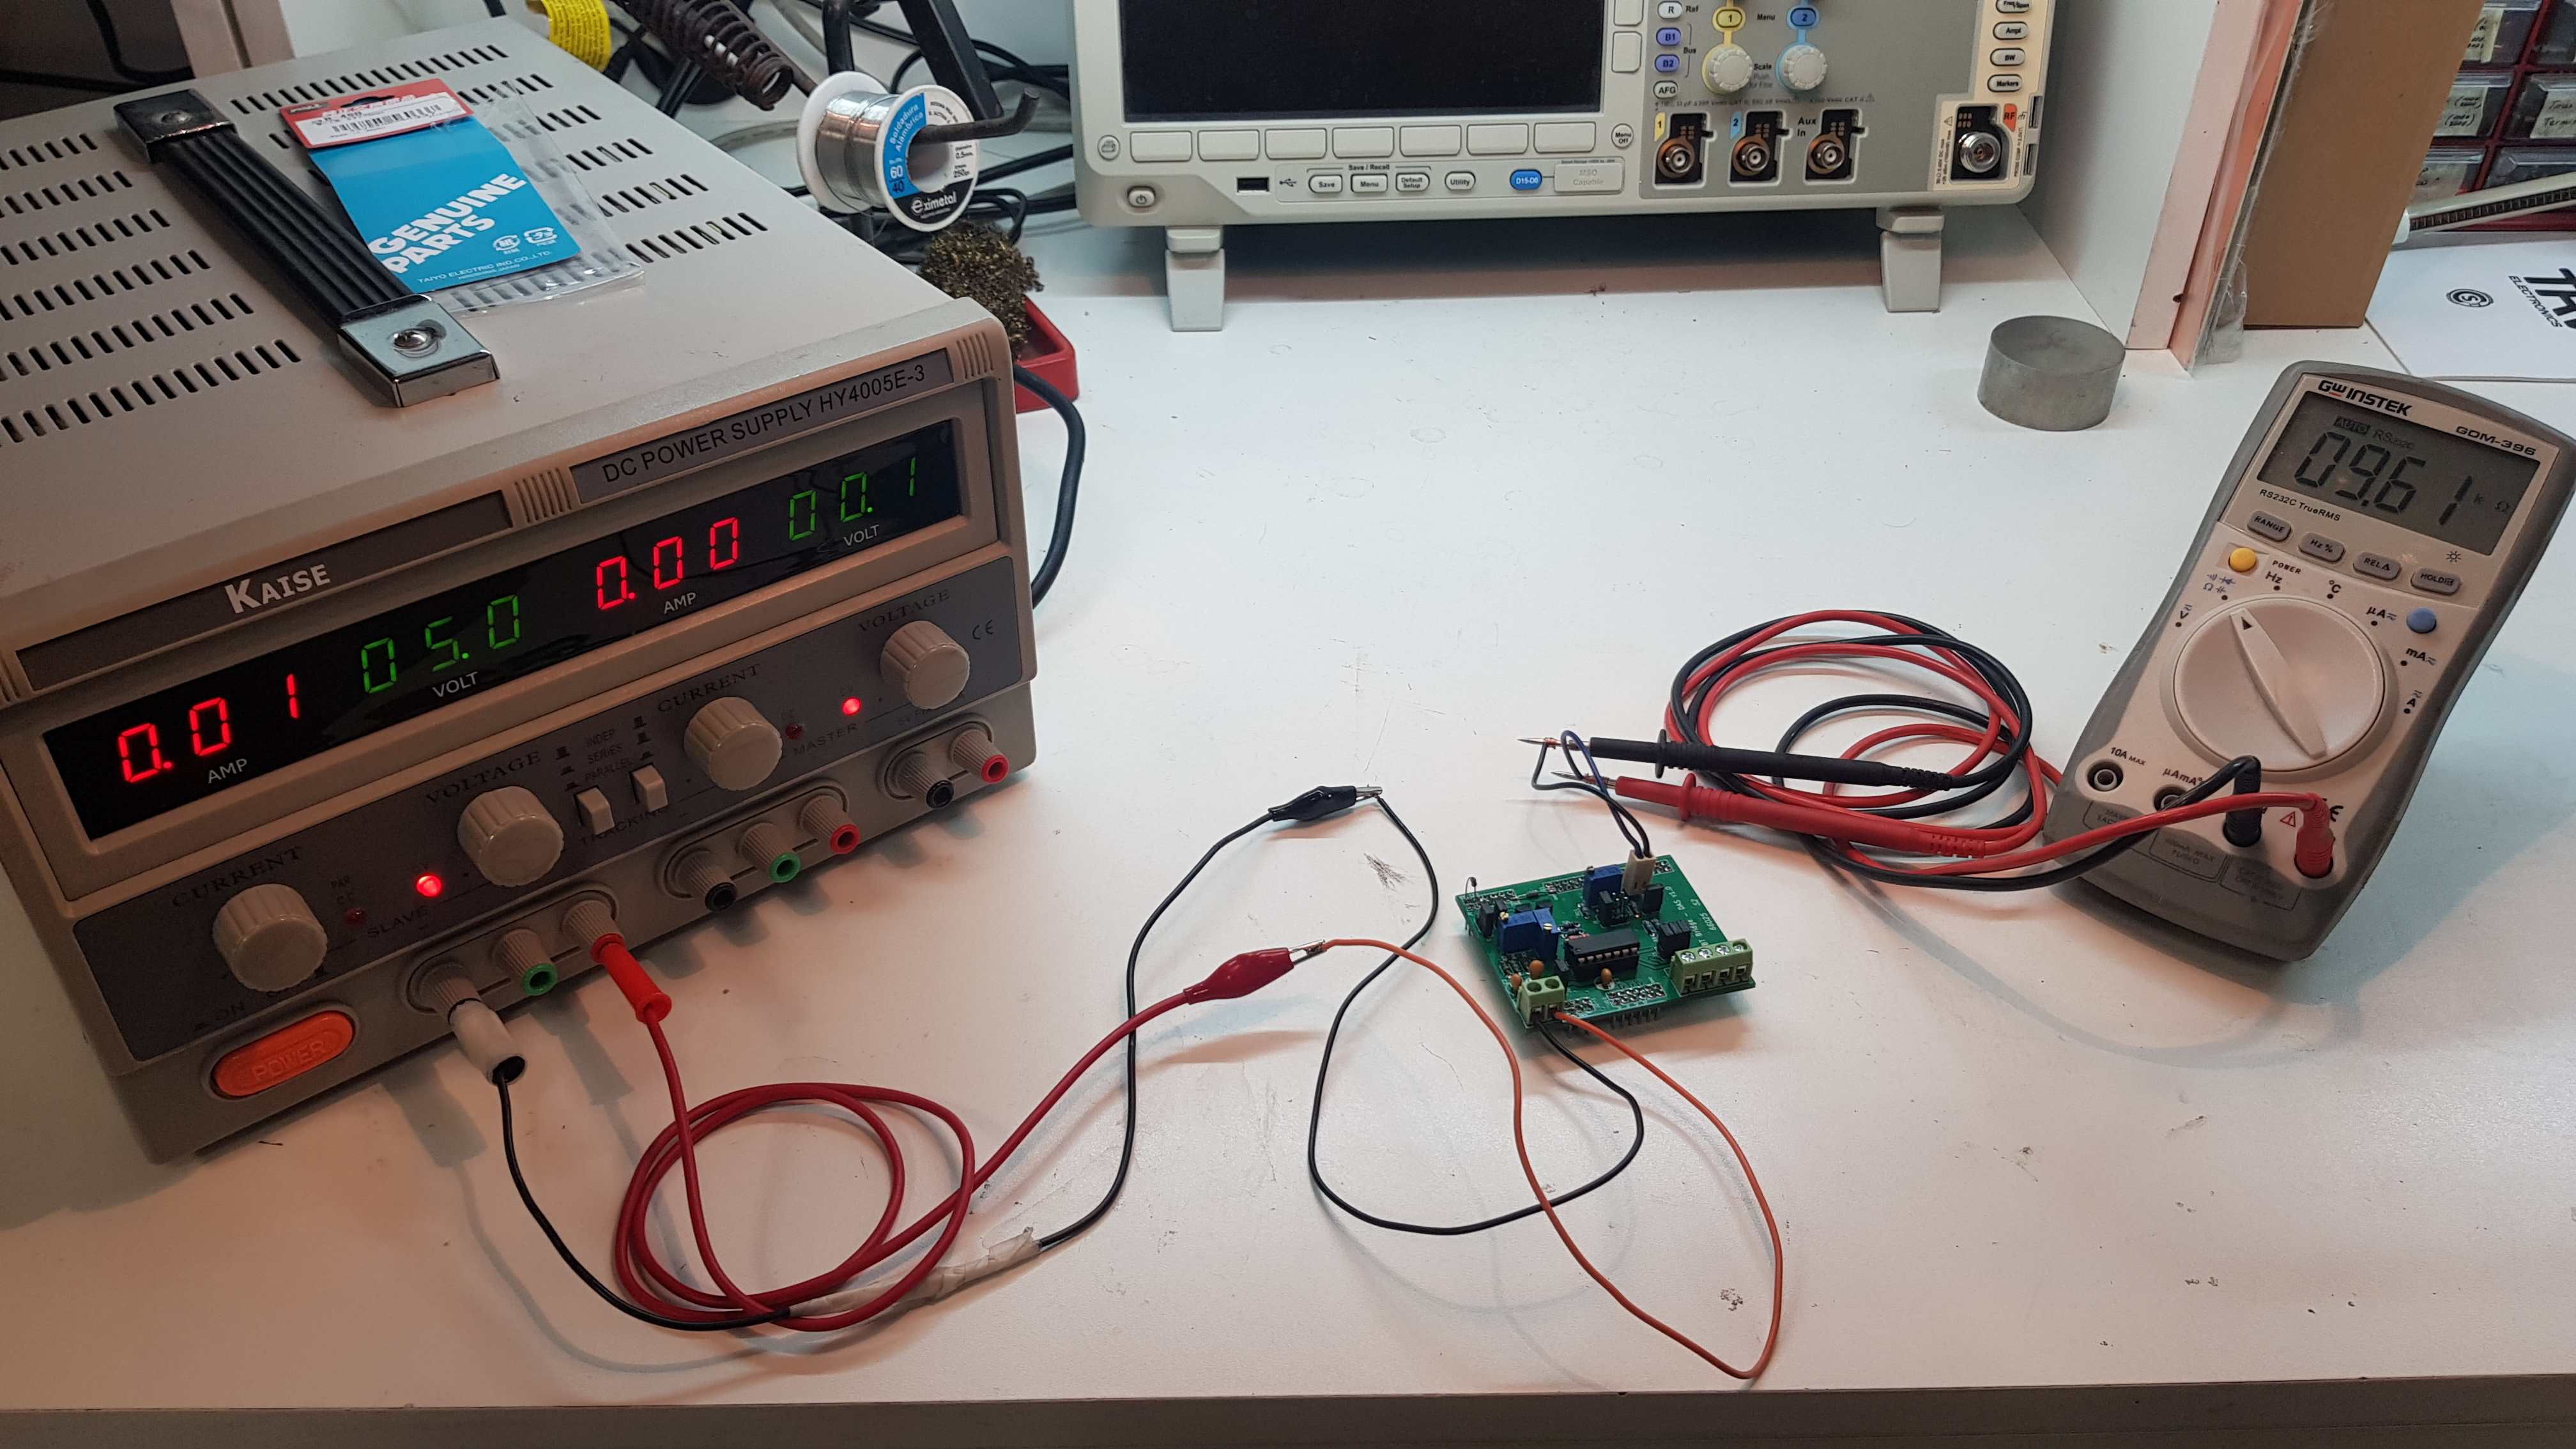
\includegraphics[width=\textwidth]{graficos/banco_experimental.jpg}
	\caption{Banco experimental para ensayar el prototipo de la soluci�n circuital de dos fuentes de corriente.}
	\label{fig:banco_exp}
\end{figure}


\subsection{An�lisis de incertezas en la determinaci�n de $R_\text{th}$}

Una de las caracter�sticas fundamentales del registrador SIPPICAN es su baja incerteza, establecida en $\pm 0.2\:^\circ\text{C}$. La obtenci�n de una medici�n de temperatura a trav�s de la estimaci�n de la resistencia del termistor de un XBT, $R_\text{th}$, con una tolerancia menor o igual que la lograda por el registrador original impone requerimientos de incerteza m�xima para su determinaci�n. 

Observando el comportamiento de la resistencia del termistor en funci�n de la temperatura, expuesto en la FIG. \ref{fig:transferenciaXBT}, es posible establecer una cota m�xima para la incerterza relativa en la determinaci�n de $R_\text{th}$, como la menor de las incertezas relativas para todo el rango de funcionamiento. Esta cota se ubica en torno al 0.8 \%. Aplicando teor�a de propagaci�n de errores al estimador $\tilde{R}_\text{th}$, descripto a partir de la Ec. \eqref{ec:Rth_monio}, se obtiene:

\begin{equation}
\varepsilon_{\tilde{R}_\text{th}} = \varepsilon_{V_\text{AB}} + \varepsilon_{V_\text{ai1,ai3}} + \varepsilon_{R_\text{aux}}
\end{equation}

\noindent donde cada t�rmino representa la incerteza relativa vinculada a cada una de las variables que determinan el valor de $\tilde{R}_\text{th}$. Las incertezas de cada variable deben ser tales que su suma sea menor que 0,8 \%. La incerteza $\varepsilon_{R_\text{aux}}$ puede establecerse en torno al 0,1 \% si se utilizan resistores de precisi�n. Las tensiones $V_\text{AB}$ y $V_\text{ai1,ai3}$ se obtienen restando tensiones en nodos individuales respecto del nodo com�n, las cuales se registran a trav�s de las entradas anal�gicas del circuito digitalizador. 

Las entradas de un conversor A/D tienen una incerteza absoluta que es caracter�stica del microprocesador utilizado, y  depende del modo de funcionamiento, el rango de tensiones m�ximas con el cual digitaliza y de las caracter�sticas del circuito impreso en el que est� montado. 

Para el kit de desarrollo propuesto, que est� provisto de conversores A/D de 12 bits, es posible establecer la incerteza absoluta de una medici�n individual en 4 cuentas (o bits menos significativos, LSBs) \citep{AN4073}, que, para una tensi�n de alimentaci�n del microprocesador de 3,3 V, se traduce en una dispersi�n de 3,22 mV. Esto conduce a incertezas absolutas, para mediciones diferenciales, de 6,44 mV.

% =====================================================================================================
% =====================================================================================================
% P�GINA DE REFERENCIAS
% =====================================================================================================
% =====================================================================================================

\clearpage

\addcontentsline{toc}{section}{REFERENCIAS}
\bibliographystyle{apa-good}	% (uses file "plain.bst")
\bibliography{7_Referencias}	% Ac� est� la base de datos de referencias. Espera el archivo "7_Referencias.bib"

\clearpage

% =====================================================================================================
% =====================================================================================================
% AP�NDICE
% =====================================================================================================
% =====================================================================================================


% Reseteo y cambio de numeraci�n para los ap�ndices
\setcounter{section}{0}
\renewcommand\appendix{\Roman{section}}
%\def\thesection{\Roman{section}}

\appendix
\appendixpage
\addappheadtotoc
\section{Circuito esquem�tico completo del puente de medici�n.}
\label{ApendiceA}


\begin{landscape}
\begin{figure}[htpb]
\centering 
\vspace{2cm}
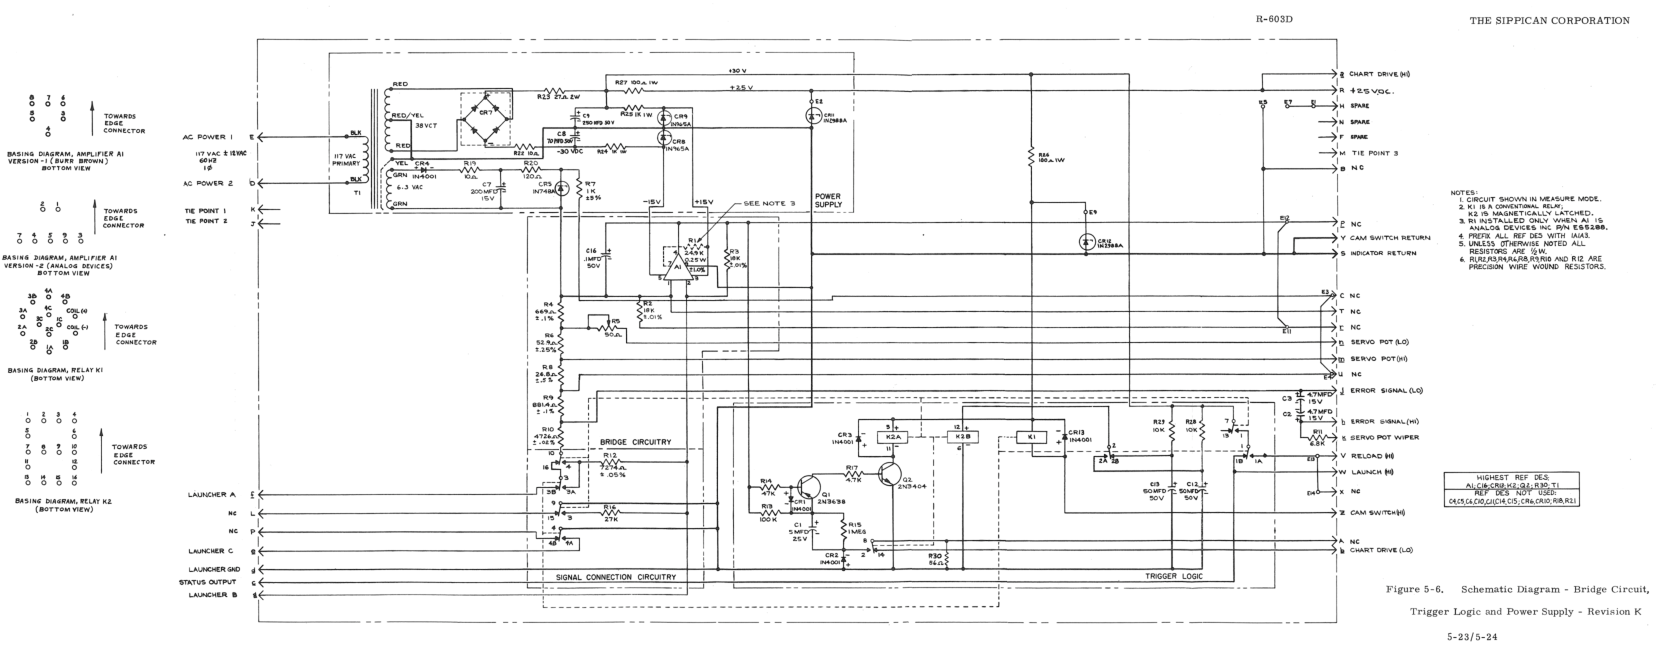
\includegraphics[height=.65\textheight]{./graficos/Esquematico_puente_recortado.pdf}
%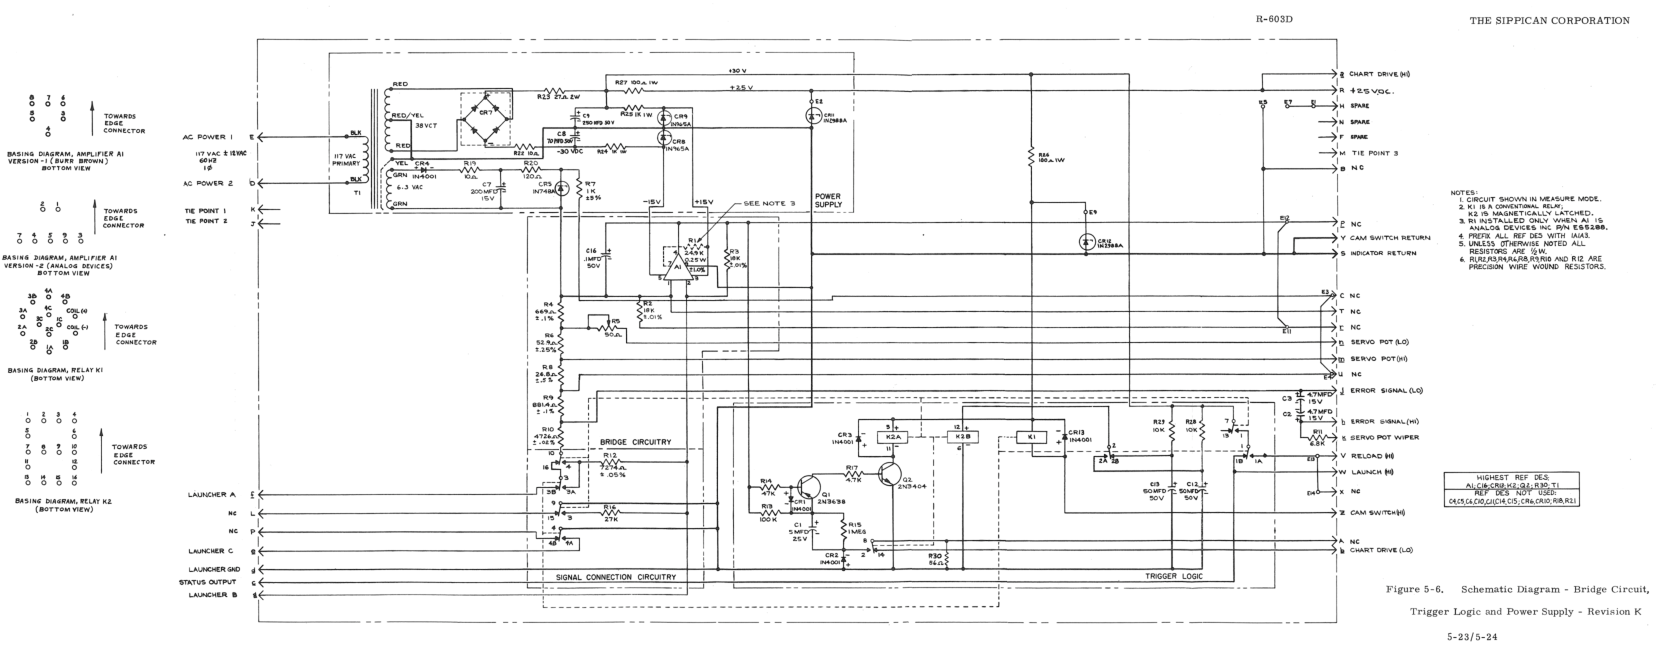
\includegraphics[width=1\textwidth]{./graficos/Esquematico_puente_recortado.pdf}
\caption{Circuito esquem�tico completo del puente de medici�n del registrador Sippican MK 2A-1.}
\label{fig:circuito_puente}
\end{figure}



\end{landscape}


\end{document}
